
% ----------------------------------------------------------------------
%                   LATEX TEMPLATE FOR PhD THESIS
% ----------------------------------------------------------------------

% based on Harish Bhanderi's PhD/MPhil template, then Uni Cambridge
% http://www-h.eng.cam.ac.uk/help/tpl/textprocessing/ThesisStyle/
% corrected and extended in 2007 by Jakob Suckale, then MPI-CBG PhD programme
% and made available through OpenWetWare.org - the free biology wiki


%: Style file for Latex
% Most style definitions are in the external file PhDthesisPSnPDF.
% In this template package, it can be found in ./Latex/Classes/
\documentclass[twoside,11pt]{Latex/Classes/PhDthesisPSnPDF}


%: Macro file for Latex
% Macros help you summarise frequently repeated Latex commands.
% Here, they are placed in an external file /Latex/Macros/MacroFile1.tex
% An macro that you may use frequently is the figuremacro (see introduction.tex)
% This file contains macros that can be called up from connected TeX files
% It helps to summarise repeated code, e.g. figure insertion (see below).

% insert a centered figure with caption and description
% parameters 1:filename, 2:title, 3:description and label
\newcommand{\figuremacro}[3]{
	\begin{figure}[htbp]
		\centering
		\includegraphics[width=1\textwidth]{#1}
		\caption[#2]{\textbf{#2} - #3}
		\label{#1}
	\end{figure}
}

% insert a centered figure with caption and description AND WIDTH
% parameters 1:filename, 2:title, 3:description and label, 4: textwidth
% textwidth 1 means as text, 0.5 means half the width of the text
\newcommand{\figuremacroW}[4]{
	\begin{figure}[htbp]
		\centering
		\includegraphics[width=#4\textwidth]{#1}
		\caption[#2]{\textbf{#2} - #3}
		\label{#1}
	\end{figure}
}

% inserts a figure with wrapped around text; only suitable for NARROW figs
% o is for outside on a double paged document; others: l, r, i(inside)
% text and figure will each be half of the document width
% note: long captions often crash with adjacent content; take care
% in general: above 2 macro produce more reliable layout
\newcommand{\figuremacroN}[3]{
	\begin{wrapfigure}{o}{0.5\textwidth}
		\centering
		\includegraphics[width=0.48\textwidth]{#1}
		\caption[#2]{{\small\textbf{#2} - #3}}
		\label{#1}
	\end{wrapfigure}
}

% predefined commands by Harish
\newcommand{\PdfPsText}[2]{
  \ifpdf
     #1
  \else
     #2
  \fi
}

\newcommand{\IncludeGraphicsH}[3]{
  \PdfPsText{\includegraphics[height=#2]{#1}}{\includegraphics[bb = #3, height=#2]{#1}}
}

\newcommand{\IncludeGraphicsW}[3]{
  \PdfPsText{\includegraphics[width=#2]{#1}}{\includegraphics[bb = #3, width=#2]{#1}}
}

\newcommand{\InsertFig}[3]{
  \begin{figure}[!htbp]
    \begin{center}
      \leavevmode
      #1
      \caption{#2}
      \label{#3}
    \end{center}
  \end{figure}
}


%%% Local Variables: 
%%% mode: latex
%%% TeX-master: "~/Documents/LaTeX/CUEDThesisPSnPDF/thesis"
%%% End: 

\usepackage[T1]{fontenc}
\usepackage{array}
\usepackage{pdfpages}
% \usepackage{nomencl}
\usepackage{adjustbox}
\usepackage{algorithmic}
\usepackage{amsmath,amssymb,amsfonts}
%\usepackage[backend=bibtex,style=ieee]{biblatex}
%\usepackage{bookmark}
\usepackage{tabularx,array}
\usepackage{booktabs}
\usepackage{caption}
% \usepackage{cite}
\usepackage{color}
\usepackage[inline]{enumitem}
\usepackage{float}
\usepackage[T1]{fontenc}
%\usepackage{fontspec}
\usepackage{svg}
\usepackage{footnote}
\usepackage{graphicx}
% \usepackage[colorlinks=true,citecolor=blue]{hyperref}
% \usepackage{inputenc}[utf8]
\usepackage{listings}
% \usepackage{textcomp}
\usepackage[flushleft]{threeparttable}
% \usepackage{subcaption}
\usepackage{xcolor}
\usepackage{cleveref}
\usepackage{csquotes}

% \makenomenclature

% ------------------------------------------------------------------------%
% Proper Python Syntax Highlighting                                       %
% Author: redmode
% https://tex.stackexchange.com/questions/83882/how-to-highlight-python   %
% -syntax-in-latex-listings-lstinputlistings-command#83883                %
% ----------------------------------------------------------------------- %

% Default fixed font does not support bold face
\DeclareFixedFont{\ttb}{T1}{txtt}{bx}{n}{8} % for bold
\DeclareFixedFont{\ttm}{T1}{txtt}{m}{n}{8}  % for normal

% Custom colors
\definecolor{deepblue}{rgb}{0,0,0.5}
\definecolor{deepred}{rgb}{0.6,0,0}
\definecolor{deepgreen}{rgb}{0,0.5,0}

% Python style for highlighting
\newcommand\pythonstyle{
	\lstset{
		language=Python,
		basicstyle=\ttm,
		showstringspaces=false,
		tabsize=4,
		aboveskip=0.2cm,
		belowskip=0.2cm,
		otherkeywords={self},             % Add keywords here
		keywordstyle=\ttb\color{deepblue},
		emph={MyClass,__init__},          % Custom highlighting
		emphstyle=\ttb\color{deepred},    % Custom highlighting style
		stringstyle=\color{deepgreen},
		frame=tb,                          % Any extra options here
		prebreak=\textbackslash,
		linewidth=8.85cm,
		breaklines=true,
	}
}

% Python environment
\lstnewenvironment{python}[1][] {
	\pythonstyle\lstset{#1}
}{}

% Python for inline
\newcommand\pythoninline[1]{{\pythonstyle\lstinline!#1!}}

% Python for external file
\newcommand\pythonexternal[2][]{{\pythonstyle\lstinputlisting[#1]{#2}}}

% ----------------------------------------------------------------------- %

% Bash style for highlighting
\newcommand\bashstyle{
	\lstset{
		language=Bash,
		basicstyle=\ttm,
		showstringspaces=false,
		tabsize=2,
		%commentstyle=itshape,
		aboveskip=0.2cm,
		belowskip=0.2cm,
		prebreak=\textbackslash,
		extendedchars=true,
		mathescape=false,
		% literate= {\$}{{\textcolor{blue}{\$}}}1 {&}{{\textcolor{blue}{\&}}}1 {/n}{{\textcolor{green}{\textbackslash n}}}1,
		linewidth=16.35cm,
		breaklines=true
	}
}

% Bash environment
\lstnewenvironment{bash}[1][] {
	\bashstyle\lstset{#1}
}{}

% Bash for inline
\newcommand\bashinline[1]{{\bashstyle\lstinline!#1!}}

% Bash for external file
\newcommand\bashexternal[2][]{{\bashstyle\lstinputlisting[#1]{#2}}}


% Python style for highlighting
\newcommand\cstyle{
	\lstset{
		language=c,
		basicstyle=\ttm,
		showstringspaces=false,
		tabsize=4,
		aboveskip=0.2cm,
		belowskip=0.2cm,
		otherkeywords={self},             % Add keywords here
		keywordstyle=\ttb\color{deepblue},
		emph={MyClass,__init__},          % Custom highlighting
		emphstyle=\ttb\color{deepred},    % Custom highlighting style
		stringstyle=\color{deepgreen},
		frame=tb,                          % Any extra options here
		prebreak=\textbackslash,
		linewidth=16.35cm,
		breaklines=true,
	}
}

% Python environment
\lstnewenvironment{clist}[1][] {
	\cstyle\lstset{#1}
}{}

% Python for inline
\newcommand\cinline[1]{{\cstyle\lstinline!#1!}}

% Python for external file
\newcommand\cexternal[2][]{{\cstyle\lstinputlisting[#1]{#2}}}

% ----------------------------------------------------------------------- %

%: ----------------------------------------------------------------------
%:                  TITLE PAGE: name, degree,..
% ----------------------------------------------------------------------
\usepackage{graphicx}

      \textwidth 15cm
      \textheight 22cm
      \parindent 10pt
      \oddsidemargin 0.85cm
      \evensidemargin 0.37cm


\begin{document}

\thispagestyle{empty}

\begin{center}

Vrije Universiteit Amsterdam \hspace*{2cm} Universiteit van Amsterdam

\vspace{1mm}

\hspace*{-7.5cm}
\includegraphics[height=25mm]{0_frontmatter/figures/vu-griffioen.pdf}

\vspace*{-2cm}\hspace*{7.5cm}
\includegraphics[height=15mm]{0_frontmatter/figures/uva_logo.jpg}

\vspace{2cm}

{\Large Master Thesis}

\vspace*{1.5cm}

\rule{.9\linewidth}{.6pt}\\[0.4cm]
{\huge \bfseries OpenCSD: Log-Structured Filesystem Enabled Computational
Storage Device Platform\par}\vspace{0.4cm}
\rule{.9\linewidth}{.6pt}\\[1.5cm]

\vspace*{2mm}

{\Large
\begin{tabular}{l}
{\bf Author:} ~~Corne Lukken ~~~~ (2639319)
\end{tabular}
}

\vspace*{2cm}

\begin{tabular}{ll}
{\it 1st supervisor:}   & ~~Dr. ir. Animesh Trivedi \\
{\it daily supervisor:} & ~~Dr. ir. Animesh Trivedi \\
{\it 2nd reader:}       & ~~Prof. dr. ir. Alexandru Iosup
\end{tabular}

\vspace*{2.5cm}

\textit{A thesis submitted in fulfillment of the requirements for\\ the joint UvA-VU Master of Science degree in Computer Science}

\vspace*{1.8cm}

\today\\[4cm] % Date

\end{center}

\newpage


% ----------------------------------------------------------------------
       
% turn off those nasty overfull and underfull hboxes
\hbadness=10000
\hfuzz=50pt


%: --------------------------------------------------------------
%:                  FRONT MATTER: dedications, abstract,..
% --------------------------------------------------------------


%\language{english}


% sets line spacing
\renewcommand\baselinestretch{1.2}
\baselineskip=18pt plus1pt


%: ----------------------- generate cover page ------------------------

\begin{center}
\textit{``Software engineers are often one of the last lines of defense against potentially dangerous and unethical practices'' \\ from {\em The code I’m still ashamed of}, by Bill Sourour (2015)}
\end{center}

%: ----------------------- cover page back side ------------------------
% Your research institution may require reviewer names, etc.
% This cover back side is required by Dresden Med Fac; uncomment if needed.

\newpage
%\vspace{10mm}
%1. First Reader: Name Surname
%
%\vspace{10mm}
%2. Daily Supervisor: Name Surname
%
%\vspace{10mm}
%3. Second Reader: Name Surname
%
%\vspace{10mm}
%4. Industrial Supervisor: Name Surname
%
%\vspace{20mm}
%Day of the defense:

%\vspace{20mm}
%\hspace{70mm}Signature from head of PhD committee:



%: ----------------------- abstract ------------------------

% Your institution may have specific regulations if you need an abstract and where it is to be placed in the document. The default here is just after title.


% Thesis Abstract -----------------------------------------------------


%\begin{abstractslong}    %uncommenting this line, gives a different abstract heading
\begin{abstracts}        %this creates the heading for the abstract page

Here goes the abstract of this thesis.
\end{abstracts}
%\end{abstractlongs}


% ---------------------------------------------------------------------- 


% The original template provides and abstractseparate environment, if your institution requires them to be separate. I think it's easier to print the abstract from the complete thesis by restricting printing to the relevant page.
% \begin{abstractseparate}
%   
% Thesis Abstract -----------------------------------------------------


%\begin{abstractslong}    %uncommenting this line, gives a different abstract heading
\begin{abstracts}        %this creates the heading for the abstract page

Here goes the abstract of this thesis.
\end{abstracts}
%\end{abstractlongs}


% ---------------------------------------------------------------------- 

% \end{abstractseparate}


%: ----------------------- tie in front matter ------------------------

\frontmatter
% Thesis Dedication ---------------------------------------------------

%\begin{dedication} %this creates the heading for the dedication page

%To ...

%\end{dedication}

% ----------------------------------------------------------------------
% Thesis Acknowledgements ------------------------------------------------


% \begin{acknowledgementslong} %uncommenting this line, gives a different acknowledgements heading
% \begin{acknowledgements}      %this creates the heading for the acknowlegments

% If you find this thesis hard to read, filled with to much whitespace or
% otherwise prefer a more dense layout, an alternative version is available 
% online:

% \end{acknowledgements}
% \end{acknowledgmentslong}

% ------------------------------------------------------------------------





%: ----------------------- contents ------------------------

\setcounter{secnumdepth}{3} % organisational level that receives a numbers
\setcounter{tocdepth}{3}    % print table of contents for level 3
\tableofcontents            % print the table of contents
% levels are: 0 - chapter, 1 - section, 2 - subsection, 3 - subsection


%: ----------------------- list of figures/tables ------------------------

\listoffigures	% print list of figures

\listoftables  % print list of tables




%: ----------------------- glossary ------------------------

% Tie in external source file for definitions: /0_frontmatter/glossary.tex
% Glossary entries can also be defined in the main text. See glossary.tex
% 
% this file is called up by thesis.tex
% content in this file will be fed into the main document

% Glossary entries are defined with the command \nomenclature{1}{2}
% 1 = Entry name, e.g. abbreviation; 2 = Explanation
% You can place all explanations in this separate file or declare them in the middle of the text. Either way they will be collected in the glossary.

% required to print nomenclature name to page header
% \markboth{\MakeUppercase{\nomname}}{\MakeUppercase{\nomname}}


% ----------------------- contents from here ------------------------

\newlength{\nomenlabelindent}
\setlength{\nomenlabelindent}{13em}
\newenvironment{nomenclature2}{%
\newcommand\entry[2]{%
   \hangindent\nomenlabelindent\noindent\makebox[\nomenlabelindent][l]{##1\quad}\ignorespaces##2\par}%
   \addcontentsline{toc}{chapter}{\protect\numberline{}Glossary}%
   \section*{Glossary}}{\par\addvspace{12pt}}

\begin{nomenclature2}
    \entry{HDD}{Hard-Disk Drive} % 233
    \entry{SSD}{Solid-State Drive} % 234
    \entry{NVMe}{Non-Volatile Memory express} % 250
    \entry{FTL}{Flash Translation Layer} % 255
    \entry{CSx}{Computational Storage Device} % 257
    \entry{ISA}{Instruction Set Architecture} % 274
    \entry{eBPF}{extended Berkely Packet Filter} %293
    \entry{ZNS}{Zoned NameSpaces} % 294
    \entry{Host Managed}{Storage device that performs no automatic garbage
        collection or wear leveling exposing facilities to do so to the host} % 296
    \entry{Hybrid Filesystem}{Filesystem supporting both regular access as well
        as Computational Storage offloading} % 296
    \entry{LFS}{Log-Structured Filesystem} % 297
    \entry{FPGA}{Field-Programmable Gate Array} % 306
    \entry{PCIe}{Peripheral Component Interconnect express} % 310
    \entry{OS}{Operating System} % 324
    \entry{VFS}{Virtual FileSystem} % 326
    \entry{FUSE}{Filesystem in USErspace} % 327
    \entry{GPGPU}{General-Purpose computing on Graphics Processing Units} % introduction 149
    \entry{API}{Application Programming Interface} % introduction 150
    \entry{ABI}{Application Binary Interface} % introduction 159
    \entry{NAT}{Node Address Table} % 406
    \entry{OCSSD}{Open-Channel SSD} % relatedwork 29
    \entry{Programming Model}{See our previous survey
        \textit{Past, Present and Future of Computational Storage: A Survey} chapter 8.2 \cite{lukken2021past}} % relatedwork 48
    \entry{Degree of Programmability}{See our previous survey
        \textit{Past, Present and Future of Computational Storage: A Survey} chapter 8.2 \cite{lukken2021past}} % relatedwork 51
    \entry{RPC}{Remote Procedure Call} % relatedwork 57
    \entry{HTTP}{HyperText Transfer Protocol} % relatedwork 57
    \entry{SQL}{Structured Query Language} % relatedwork 96
    \entry{CSEE}{Computational Storage Execution Environment} % relatedwork 64
    \entry{SIT}{Segment Info Table} % relatedwork 64
    \entry{SSA}{Segment Summary Area} % relatedwork 64
    \entry{RTL}{Register-Transfer Level} % relatedwork 127
    \entry{NVMe-oF}{NVMe over Fabrics} % relatedwork 184
    \entry{MPI}{Message Passing Interface} % relatedwork 145
    \entry{HPC}{High-Performance Computing} % relatedwork 146
    \entry{CS}{Computer Science} % relatedwork 231
    \entry{POSIX}{Portable Operating System Interface} % design 101
    \entry{NIX}{A UNIX based operating system or derivative} % design 110
    \entry{PID}{Process IDentifier} % design 115
    \entry{Kernel}{Compiled binary or bytecode representation of a computational
        unit that can be submitted / scheduled for execution on accelarator type
        devices such as graphics cards or CSxs. Alternatively, resource and
        device management layer of an operating system.} % implementation 89
    \entry{EOF}{End Of File} % implementation 841
\end{nomenclature2}

% \printnomenclature

%\nomenclature{LSY}{ehbfuefebbfbjkjkebfjbfbfw} 
%\nomenclature{DEPC}{diethyl-pyro-carbonate; used to remove RNA-degrading enzymes (RNAases) from water and laboratory utensils}
%\nomenclature{DMSO}{dimethyl sulfoxide; organic solvent, readily passes through skin, cryoprotectant in cell culture}
%\nomenclature{EDTA}{Ethylene-diamine-tetraacetic acid; a chelating (two-pronged) molecule used to sequester most divalent (or trivalent) metal ions, such as calcium (Ca$^{2+}$) and magnesium (Mg$^{2+}$), copper (Cu$^{2+}$), or iron (Fe$^{2+}$ / Fe$^{3+}$)}
 

\begin{multicols}{2} % \begin{multicols}{#columns}[header text][space]
\begin{footnotesize} % scriptsize(7) < footnotesize(8) < small (9) < normal (10)

\printnomenclature[1.5cm] % [] = distance between entry and description
\label{nom} % target name for links to glossary

\end{footnotesize}
\end{multicols}



%: --------------------------------------------------------------
%:                  MAIN DOCUMENT SECTION
% --------------------------------------------------------------

% the main text starts here with the introduction, 1st chapter,...
\mainmatter

\renewcommand{\chaptername}{} % uncomment to print only "1" not "Chapter 1"


%: ----------------------- subdocuments ------------------------

% Parts of the thesis are included below. Rename the files as required.
% But take care that the paths match. You can also change the order of appearance by moving the include commands.


% this file is called up by thesis.tex
% content in this file will be fed into the main document

%: ----------------------- introduction file header -----------------------
\chapter{Introduction}

% the code below specifies where the figures are stored
\ifpdf
    \graphicspath{{1_introduction/figures/PNG/}{1_introduction/figures/PDF/}{1_introduction/figures/}}
\else
    \graphicspath{{1_introduction/figures/EPS/}{1_introduction/figures/}}
\fi

% ----------------------------------------------------------------------
%: ----------------------- introduction content ----------------------- 
% ----------------------------------------------------------------------



%: ----------------------- HELP: latex document organisation
% the commands below help you to subdivide and organise your thesis
%    \chapter{}       = level 1, top level
%    \section{}       = level 2
%    \subsection{}    = level 3
%    \subsubsection{} = level 4
% note that everything after the percentage sign is hidden from output



\section{Context} 

% We have a separate previous work section we will ignore most of the different
% related literature in the introduction.

% Problem

The amount of data being generated and processed worldwide is growing rapidly.
Meanwhile the prevelant Von Nuemann computer architecture requires all data is 
moved to system memory before it can be processed \cite{2018-neumann-bottleneck}.
Until recently storage devices such as hard-disk drives (HDDs) or solid state
drives (SSDs) have only been passively storing data. With the increasing
bandwidth persistent storage devices like SSDs achieve this excessive data
movement to memory is increasingly becoming a bottleneck \cite{2014-micro-ndp}.
Similarly, the CPU generational performance
improvements \cite{2016-western-digital} as well as link speeds of interconnects
are stagnating compared to nand flash bandwidth \cite{10.1145/3286588}, the
underlying technology enabling modern SSDs. The typical proportions of this
large bandwidth gap are demonstrated in figure \ref{figure:storagebottleneck}.

\begin{figure}
    \centering
	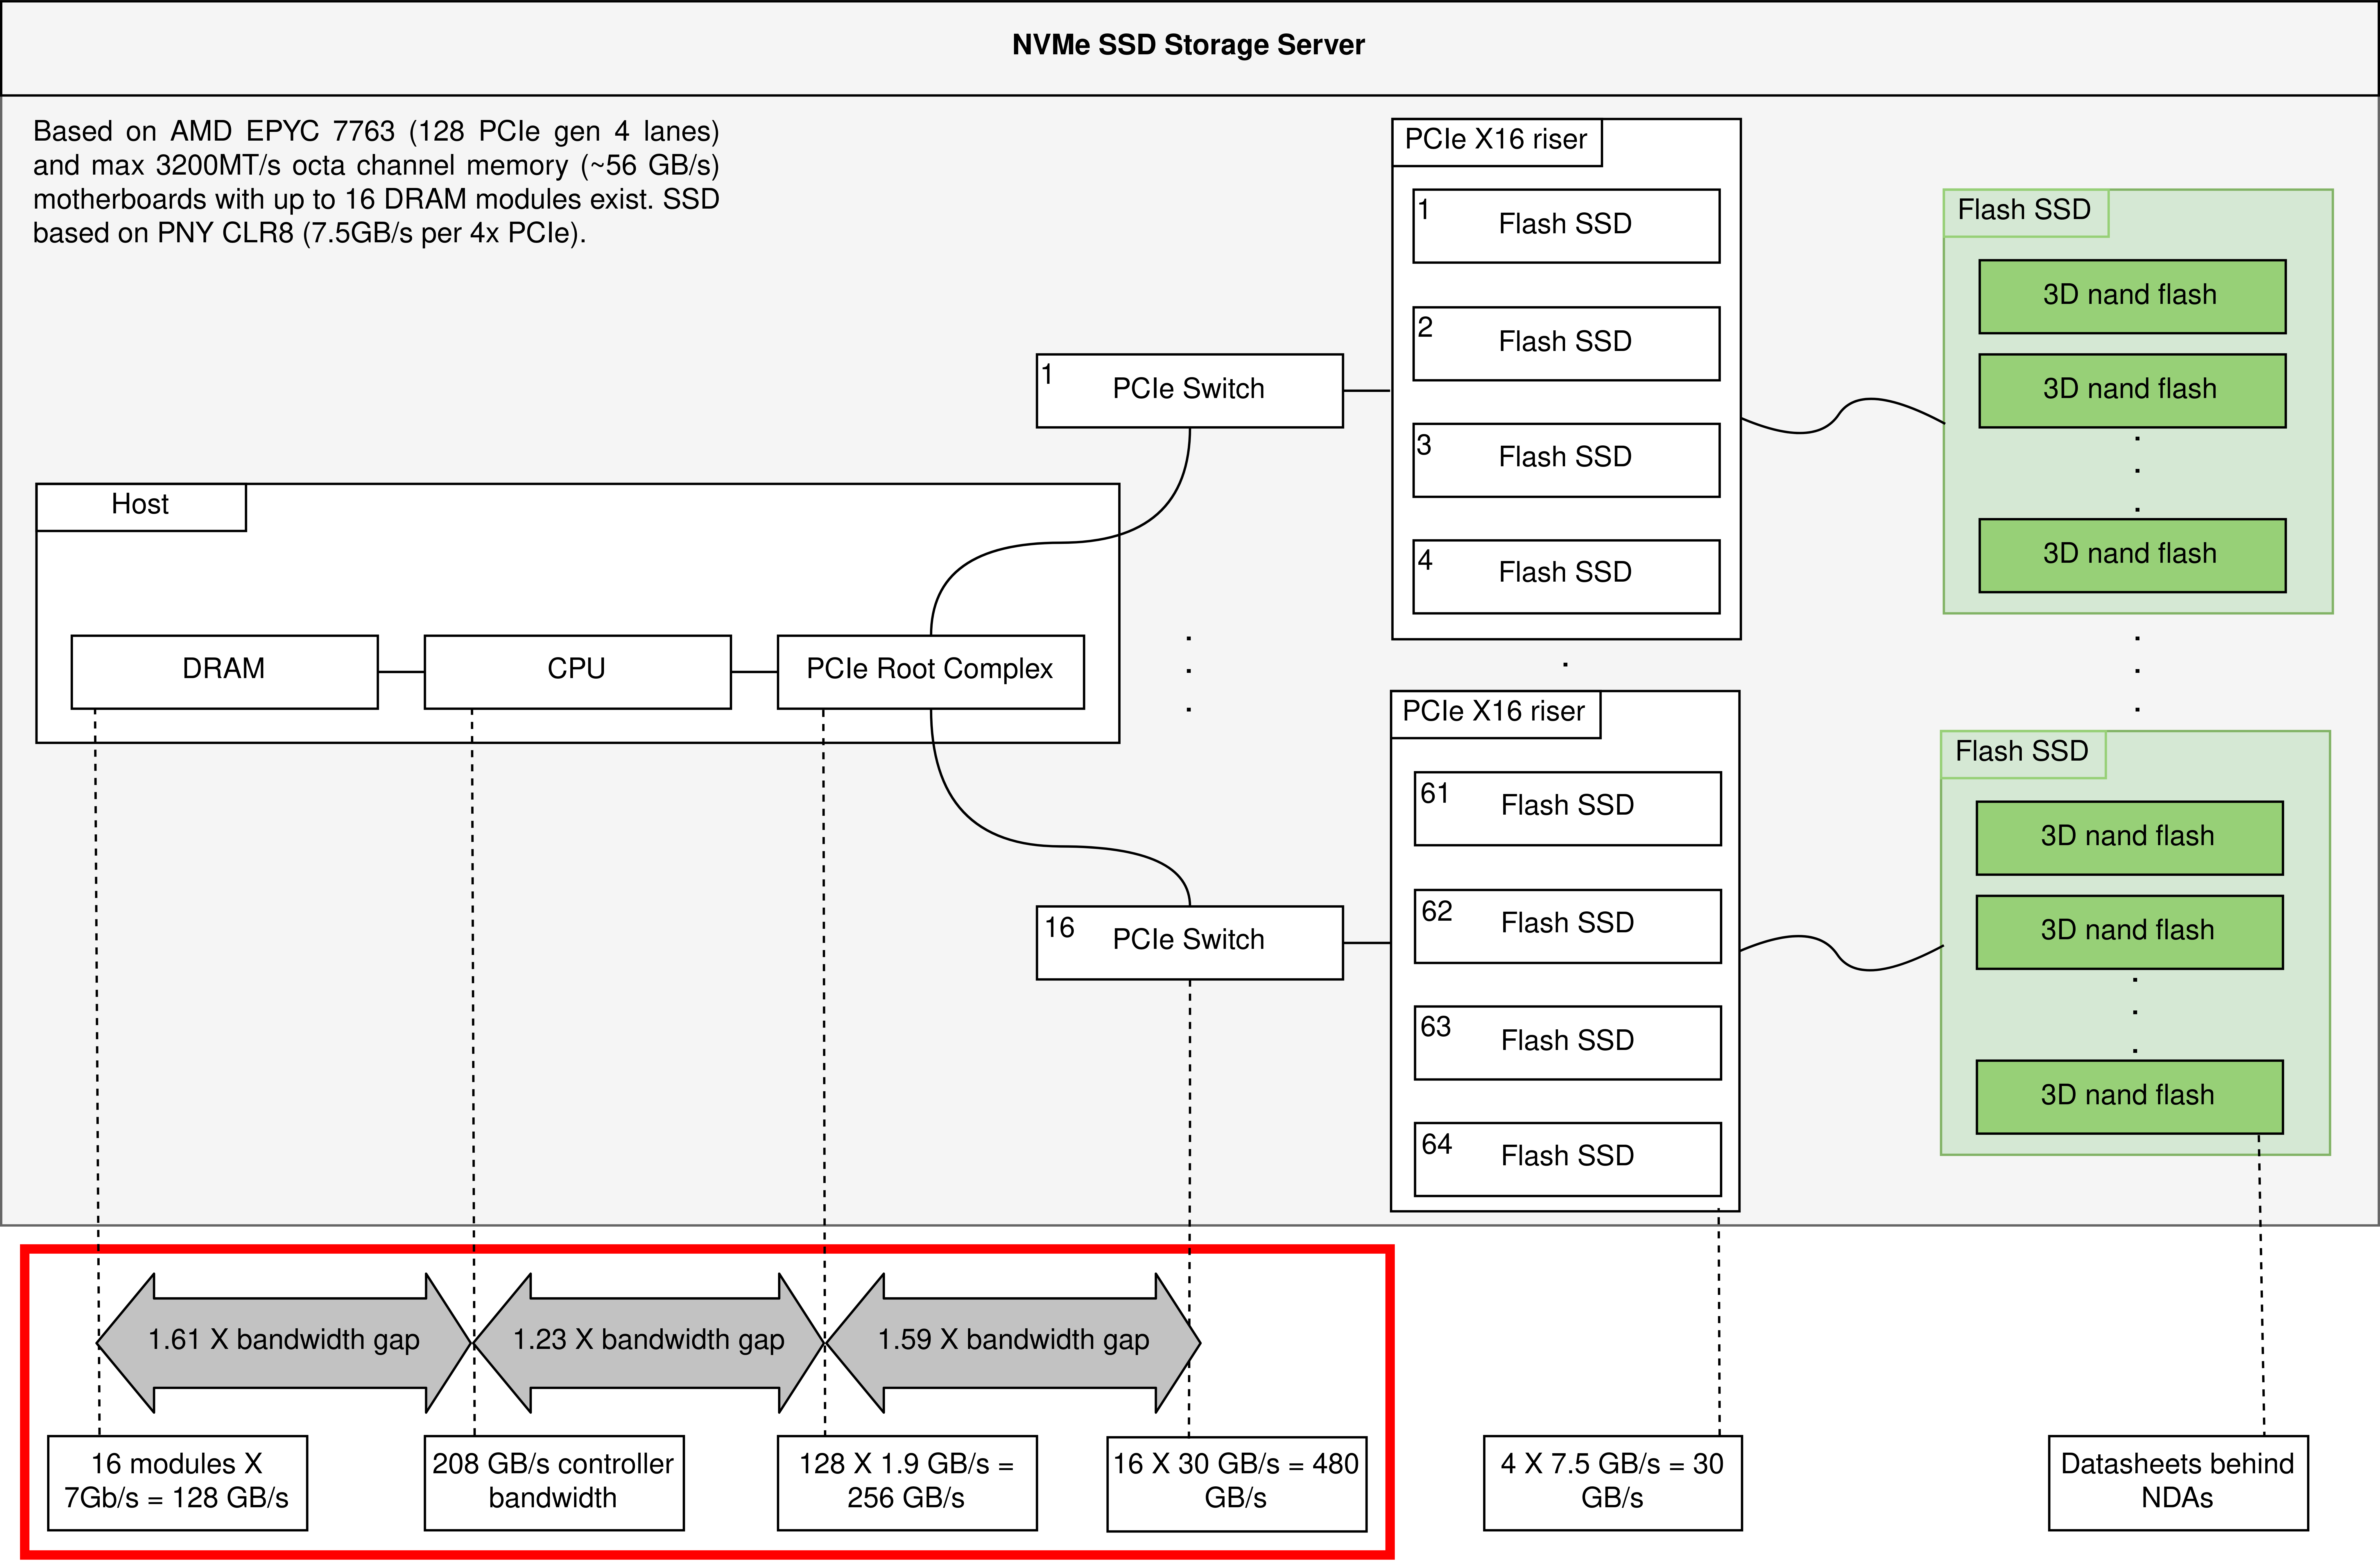
\includegraphics[width=1\textwidth]{resources/images/storage-bottleneck.png}
	\caption{Typical bandwidth limitations in modern storage servers using 64
        SSDs.}
    % \includesvg[width=0.6\columnwidth]{resources/images/module-dependencies}
    \label{figure:storagebottleneck}
\end{figure}

% Potential solution and benefits

A promising solution to this problem is the processing of data in-situ by
pushing compute to the storage layer. This solution is actively being researched
as \textit{"Programmable Storage"} and \textit{"Computational Storage"} among
other terms. The concept is not new however, as it has been previously
explored in database mainframes \cite{database-computer} as well as for
conventional HDDs \cite{active-disk-pillar, active-disks-tech,
intelligent-disk}. With rise of Non-Volatile Memory Express (NVMe) technologies
offering signifcantly more device-internal bandwidth this concept is being
revisted. What makes NVMe SSDs even more suited is that they already contain
capable processing units often boasting even multiple cores. This requirement
comes from the internal management the device has to perform known as the
\textit{Flash Translation Layer} (FTL). Devices utilizing computational elements
on conventional SSDs for \textit{Computational Storage} are commonly known as
\textit{Computational Storage Devices} (CSx)s. The potential benefits of such a
heteregenous architecture offering programmable storage include energy saving,
cost reduction and performance improvements.

% Challenges

Despite all these benefits there is still no widespread adoption even after a
decade of research \cite{lukken2021past}. A multitude of challenges
have prohibited this adoption of which several still applicable today. Four
prominent challenges include that, firstly, \textit{Computational Storage}
requires complete vertical integration. Meaning that changes are required at all
levels of abstraction, device hardware, interfaces, drivers and operating system
to name a few. Trying to integrate a solution for all levels in one prototype
results in a very large problem space. This large problem space complicates
deriving standards for designs and interfaces although the development of such a
standard by SNIA is on-going \cite{snia-model}. Secondly, vendors might choose
to use different hardware with different
\textit{Instruction Set Architectures} (ISA)s or different host-to-device
interfaces. These differences might result in incompatible user applications
across vendors hurting reusability and hindering adoption. Third, filesystems
are managed by the host operating system while the FTL is
managed by the device. Given that one is not aware of the processes within the
other, this semantic gap complicates several aspects such as consistency,
concurreny, multi-user tenancy and filesystem integration. Lastly, no
specialized filesystem designs exist that support both regular user access
concurrent with \textit{Computational Storage} offloading.

% Solutions

In this work we address each of these challenges directly and propose a
complete \textit{Computational Storage} solution that offers a filesystem
capable of concurrent multi-user tenancy with both regular and compute
offloading access (hybrid). We introduce each of the solutions briefly before
describing their complete case. Firstly, we circumvent the complexity of
complete vertical integration by creating a simulation platform on top of
QEMU \cite{qemu}. Secondly, We eliminate potential incompatibities across
vendors by using \textit{Extended Berkely Packet Filer} (eBPF) \cite{what-ebpf}
as compute kernel language. Third, We bridge the semantic gap by using \textit{
Zoned Namespaces} (ZNS) \cite{zns} SSDs which moves the FTL to the host
operating system (host-managed). Lastly, we allow for concurrent multi-user
tenancy in a \textit{Hybrid Filesystem} context by developing a specialized
\textit{Log-Structured Filesystem} (LFS) \cite{Rosenblum1992TheDA} with an
in-memory snapshot consistency model \cite{Viotti2016ConsistencyIN}. We present
this complete solution as \textit{OpenCSD} an open-source Apache 2 licensed CSx
simulation framework with accompanying filesystem called
FluffleFS \cite{qemu-csd}.

Clearly computational storage is a promising avenue to the data movement
bottleneck. However, there remain clear challenges that currently prevent it
from being effective. Having mentioned the four parts of our solution briefly we
now describe their complete cases in the next sections.

\subsection{A Case for CSx Simulation}

The lack of a standardized design has lead to a large variety of different
hardware architectures being explored including using embedded CPUs or
\textit{Field-Programmable Gate Arrays} (FPGA)s. Moreover, closed-source
devices have even become commercially available. Still there is a lot of
uncertainty about the right computational hardware models, interconnects and
interconnects their interfaces. Even though the \textit{Peripheral Component
Interconnect Express} (PCIe) interconnect and the NVMe storage interface
currently dominate modern storage devices it is unclear if their current
capabilities are sufficient to support CSxs. Meanwhile existing technologies
such as QEMU allow rapid development of new simulated hardware.

The lack of a clear standardized design combined with the ease of prototyping
designs in simulation clearly shows that choosing simulation over an actual
hardware prototype is the current logical choice.

\subsection{A Case for eBPF Programmability}

The concept of programmability provides end users the capability to run their
own provided code. With the introduction of modern \textit{Operating Systems}
(OS)s this is expected to happen in safe and dynamic manner. Programmability
can be achieved in different manners such as through the kernel in kernel
modules, with filesystems through \textit{Virtual File System} (VFS) or
\textit{Filesystem in USErspace} (FUSE) and with language runtimes such as those
in Python. In addition programmability can also target a peripherals instead of
the host directly such as is prevelant in \textit{General-Purpose computing on
Graphics Processing Units} (GPGPU) programming through \textit{Application
Programming Interfaces} (API)s like OpenCL \cite{opencl} and CUDA \cite{cuda}.
Through similar mechanisms programmability in CSxs can be achieved.

The uncertainty of the hardware design makes it unclear exactly how close to the
hardware and through which method of programmability CSxs will be effective.
Although, naturally, the closer to the actual storage the better
(Near-Data Processing). Therefor, our programmability must not be restricted or
favor a particular type.

Introducing eBPF an ISA and \textit{Application Binary Interface} (ABI) with a
large collection of toolchains and wideranging implementations
\cite{what-ebpf, McCanne1993TheBP}. These implementations range from complex
such as the one found in the Linux kernel to simple such as the one found in
uBPF \cite{ubpf}, with the key difference in complexity being the supported ABI.
Effectively, the implementation running (runtime) eBPF code decides the ABI by
tying special eBPF syscall instructions to predefined code. In addition, this
allows the user program and runtime to exchange important information such as
prominently done in Linux through eBPF maps \cite{bpf-man}. We demonstrate the
flexibility of such a vendor agnostic ABI as well as the internals of uBPF in
figure \ref{figure:ubpf-abi}.

\begin{figure}
    \centering
	\includegraphics[width=0.8\textwidth]{resources/images/ubpf-abi.pdf}
	\caption{Achieving vendor agnostic \textit{Application Binary Interfaces}
        (ABI) through uBPF.}
    % \includesvg[width=0.6\columnwidth]{resources/images/module-dependencies}
    \label{figure:ubpf-abi}
\end{figure}

The benefits of eBPF are four fold. First, the ISA is not tailored to any
specific domain and it has been used in networking \cite{xdp},
tracing \cite{enhanced-ebpf} and security \cite{seccomp} applications. Second,
the simple nature of the eBPF ISA allows for verification and bounded execution
checking such as performed by the Linux kernel \cite{kern-analysis}. Third, eBPF
supports efficient code generation through jitting achieving close to bare-metal
performance. Lastly, eBPF has been positioned as the unified ISA for
heteregenous computing \cite{Brunella2020hXDPES, bpf-uapi}.

\subsection{A Case for ZNS}

A new emerging NVMe standard is \textit{Zoned Namedspaces} (ZNS). It can been
seen as the technical successor to Open-Channel % \cite{}.
This standard allows host visibility and control over data placement
(host-managed) while more closely representing nand flash behavior. This
replacement for the traditional block interface offers reduced
write-ampplifcation, lower SSD hardware requirements and more intelligent
wear-leveling and garbage collection. However ZNS SSDs come with several
constraints such as not allowing in-place updates (append-only), using a large
collection of sectors as single erasure unit and requiring wear-leveling and
garbage collection to be explicitly programmed by the host. The fundamental
difference between conventional and ZNS SSDs is shown in figure
\ref{figure:znsvsconventional}.

\begin{figure}
    \centering
	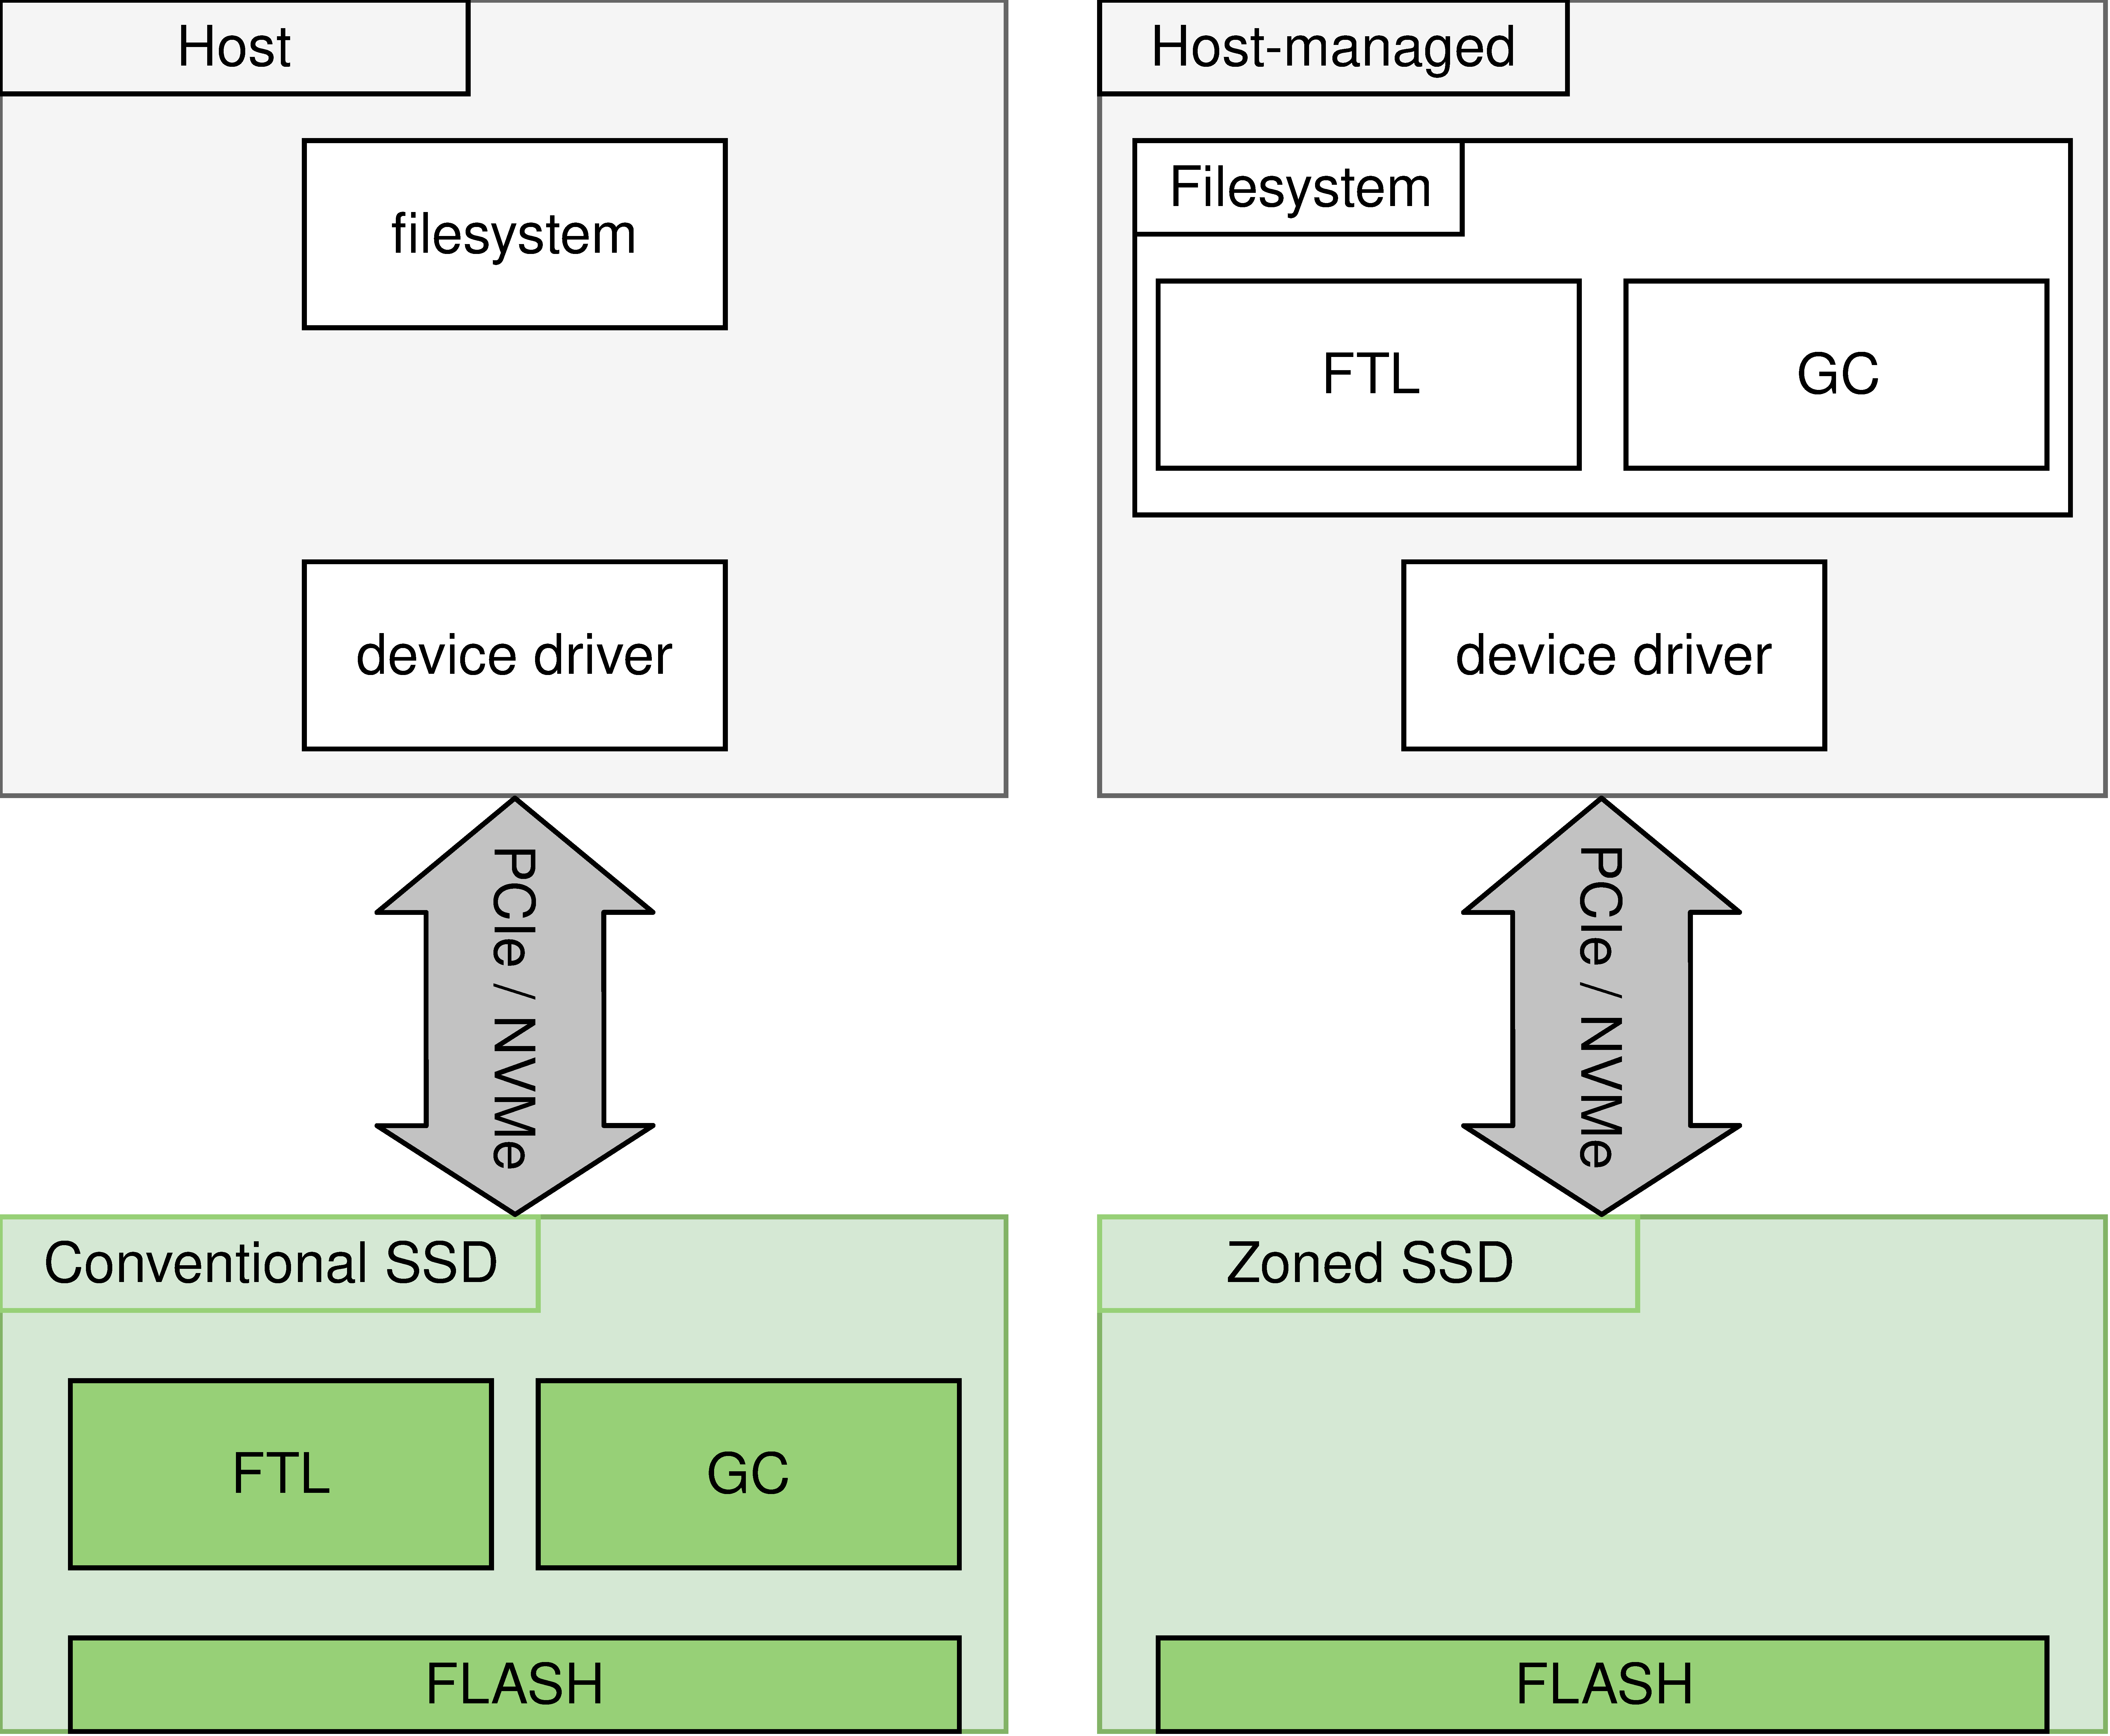
\includegraphics[width=0.6\textwidth]{resources/images/zns-vs-conventional.pdf}
	\caption{Differences between conventional and ZNS SSDs.}
    % \includesvg[width=0.6\columnwidth]{resources/images/module-dependencies}
    \label{figure:znsvsconventional}
\end{figure}

Yet we argue ZNS greatly improves the feasibility of CSx supporting
\textit{hybrid filesystems}. Firstly, ZNS offers more predictable performance in
conjuction with \textit{Log-Structured Filesystems} as the absence of a device
FTL means the behavior of \textit{append-only} writes won't be influenced by
underlying write-amplification or garbage-collection. Secondly, the direct
relationship between dimensions as reported to the host and to those known on
the device results in a greatly simplified exchange of information from host
submitted compute kernels as well as reduced kernel runtime translations.
Finally, this reduced semantic gap between the host and device is essential to
compute kernels running autonomously and without shared virtual memory.

\subsection{A Case for LFS}

\textit{Log-Structured Filesystems} have been around for a long
time \cite{Rosenblum1992TheDA} but have not really been popularized until the
recent advancement of nand flash. A LFS maintains one or multiple logs which
are append-only sections of the filesystem. This has the advantage of the
underlying device receiving filesystem writes as sequential I/O operations,
which is known to improve performance. In addition, LFSs are often relatively
easy to implement. Unfortunately, LFSs suffer from write-amplification because
modifcations updating inode or other data location information travels up the
chain in history. The specific type of write-amplifiction common in LFSs is
also known as the wandering tree problem. An example of write-amplification is
shown in figure \ref{figure:writeamplification}.

\begin{figure}
    \centering
	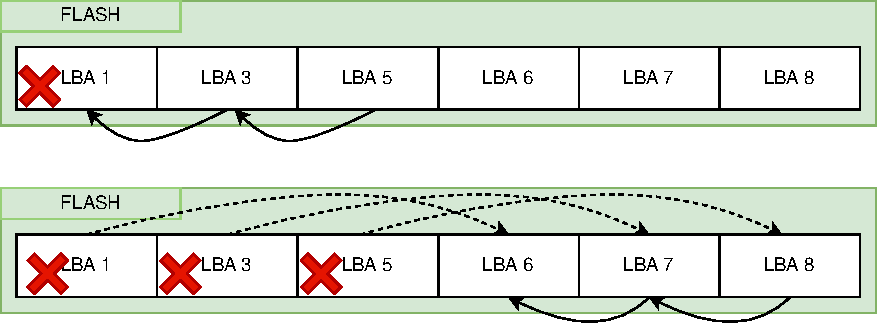
\includegraphics[width=0.7\textwidth]{resources/images/write-amplification.pdf}
	\caption{Example of write-amplification where a single invalidation leads
    to multiple linked blocks being rewritten.}
    % \includesvg[width=0.6\columnwidth]{resources/images/module-dependencies}
    \label{figure:writeamplification}
\end{figure}

Yet we argue an LFS is essential for an effective \textit{hybrid filesystem} due
to the following three reasons. Firstly, the append-only nature of a LFS is the
best fit for the append-only requirement of ZNS SSDs. Secondly, the
chronological order of logs allows for snapshotting, versioning and simplified
crash recovery. It is thanks to the properties of an LFS that FluffleFS is able
to provide in-memory snapshots to compute kernels. Lastly, the problem around
write-amplification is a solved issue thanks to the F2FS \cite{Lee2015F2FSAN}
work which introduced a so called \textit{Node Address Table} (NAT). A diagram
showing a simplified view of F2FS and the NAT is shown in figure
\ref{figure:f2fsnat}.

\begin{figure}
    \centering
	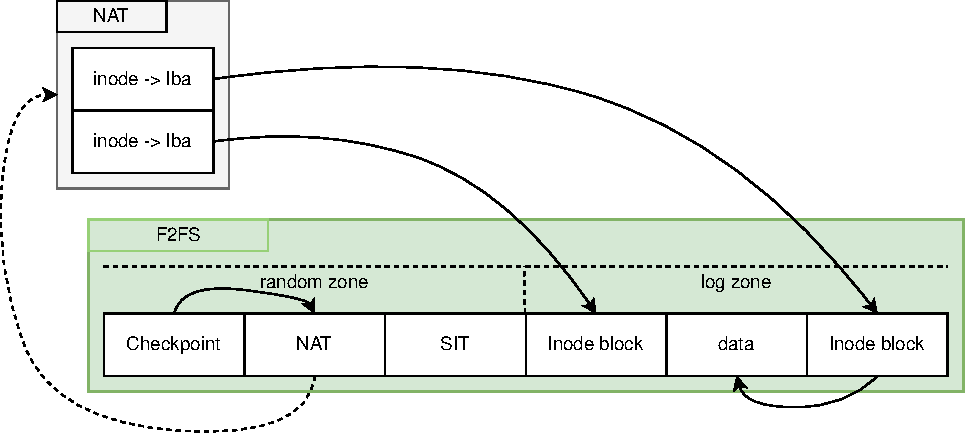
\includegraphics[width=0.7\textwidth]{resources/images/f2fs-nat.pdf}
	\caption{Overcoming LFS limitations with a separate random zone and NAT.}
    % \includesvg[width=0.6\columnwidth]{resources/images/module-dependencies}
    \label{figure:f2fsnat}
\end{figure}

As shown each of these cases demonstrates the importance of each part. Only
together are they able to provide a complete solution for open research
questions given the current state of the field as we will proof in the design
section.

\section{Research Question}

In this section we formulate the main scientific contribution of this work in
the form of a research question. In addition, we formulate several sub questions
which aid in showing to which extend the main research question is answered.
The sub research questions relate both to design choices as well as qualitative
performance evaluations.

Our main scientific contribution aims to answer one of the most prominent open
research questions in the field of Computational Storage. The question of
designing a filesystem that supports both regular and offloaded access, so
called \textit{hybrid filesystems}. We formulate that into the following
research question. Namely,

\begin{displayquote}
    How to create a multi-user tenant (hybrid) LFS with Computational Storage
    offloading support?
\end{displayquote}

\subsection{Sub Questions}

% Ensure the research questions are such that they support the design
% requirements.

\begin{itemize}
    \item Design Requirements
    \begin{enumerate}
        \item What existing technologies are best suited for a hybrid LFS?
        \item What techniques can be used to minimize the complexity required to
              use a hybrid LFS?
        \item What mechanisms allow for simplified replacement of used existing
              technologies in a hybrid LFS?
        \item How to register CSx compute kernels using existing operating 
              system APIs?
        \item How to differentiate individual users, files and I/O operations in
              relation to their CSx compute kernel?
        \item How to ensure user submitted CSx compute kernels are safe?
    \end{enumerate}
    \item Experimental Evaluation
    \begin{enumerate}
        \item Can a multi-user tenant hybrid LFS achieve unstagnated performance
              for concurrent regular and offloaded file access?
        \item Can a multi-user tenant hybrid LFS reduce the data movement
              between device and host?
        \item Can a multi-user tenant hybrid LFS reduce the host load for
              asynchronous applications?
    \end{enumerate}
\end{itemize}

Our design requirements aim to result in practical solution that can easily be
adopted should new technologies emerge with high ease of use while actually
allowing for concurrent regular and offloaded access. In addition, our
experimental evaluation aims to show that while doing so we can achieve the
expected benefits of such designs.

\section{Research Method}

A well defined research method is needed to answer the main, design requirements
and performance evaluation research questions. Given the nature of the work,
being the development and evaluation of a research software prototype, an
iterative design approach simular to that of Agile is best suited.

\subsection{Design Approach}

Our design approach consist of an initial step performed only once followed by
as many iterations as necessary to complete the design. The first being
identifying the critical components. Subsequently, the iterative design approach
consist of the following three steps. First, we identify existing technologies
that can be used for one or more of the critical components. Secondly, we
evaluate each of the potential technologies. Third, we implement the
functionality of the component using the selected techology. Any issue that
prevents the further use of a chosen technology starts the next iteration of the
design process. If no alternatives can be found workarounds or practical
limitations are introduced instead.

This design approach should allow for the selection of the best available
existing technologies given the design requirements while allowing to change
any chosen technologies during the implementation process.

\subsection{Evaluation Approach}

%  Iterative design approach


% this file is called up by thesis.tex
% content in this file will be fed into the main document

\chapter{Related Work} % top level followed by section, subsection


% ----------------------- paths to graphics ------------------------

% change according to folder and file names
\ifpdf
    \graphicspath{{7/figures/PNG/}{7/figures/PDF/}{7/figures/}}
\else
    \graphicspath{{7/figures/EPS/}{7/figures/}}
\fi


% ----------------------- contents from here ------------------------
% 

\section{Support Technologies}

Several developments across different fields have been essential for the
goals we envision for CSx. In this section we go to the most prominent of 
these developments. However, only developments not directly related to CSx are
covered as the next section covers these CSx developments detail.

\section{Computational Storage Devices}

While OpenCSD is unique it is by no means the first CSx prototype as there
has been over a decade of research in this field \cite{lukken2021past}. In this
decade we have seen a large variety of approaches, problem spaces, hardware
platforms and software APIs. There is significant progression in this field, 
however, several important challenges are still open research
questions \cite{barbalacecomputational}.

In this section we introduce characteristics of CSx prototypes, the most
prominent open research questions, provide an overview of notable works,
describe the progression of the field and describe fundamentally missing
features that hinder adoption and widespread use of CSxs.

% Introduce early working prototypes

% Demonstrate different hardware platforms, embedded CPU, vs FPGA.

% List of BPF using storage literature (Blockndp:, Extos: Data-centric
%extensible os, Ex-tension framework for file systems in user space, 
%  Safe and efficient remote application code execu-tion on disaggregated NVM,
% BPF for storage: an exokernel-inspired approach )

% Introduce previous ZCSD table but extended

\subsection{CSx characterstics}

There are four types of characteristics that set CSxs apart. First there is
the end user \textit{programming model}, the model of programming developers
have to use in order to interact with CSx. Second, there is the execution
environment, the level of software abstraction the end user programs are run on
(on the device). Third, is the \textit{degree of programmability}, the amount of
programming control offered to the end user. Lastly, there is the interface used
to connect the device to the host.

With end user programming models there are, in no particular order,
\textit{Dataflow (MapReduce, DAG)}, \textit{Client / Server
(RPC \footnotemark[1], HTTP \footnotemark[2])}, \textit{Shared memory} and
\textit{Declarative (Regex, MySQL)}. Although simple categories, the correct
attribution of these categories can become quite complicated due to nuances. For
instance, if an end user needs to link to a new shared library to call methods
with MySQL queries as argument it becomes unclear what the programming model
should be. In this work we argue \textit{Shared memory} as the library that
needs to be linked is introduced in the work.

\footnotetext[1]{\textit{Remote Procedure Call} (RPC)}

\footnotetext[2]{\textit{HyperText Transfer Protocol} (HTTP)}

In \textit{Computational Storage Execution Environments} (CSEE) we effectively
observe seven distinct levels of abstraction. These range from
\textit{Register-Transfer Level} (RTL) design such as using languages like
Verilog or VHDL to virtual machines. The compiled output of RTL designs is known
as a bitstream and typically programmed into an FPGA at runtime. The distinct
levels are listed below.

\begin{enumerate}
    \item Bistream; bitstream programmed directly unto FPGA.
    \item Embedded; single program, single memory space, no OS just 'real mode'.
    \item Accelerators; OpenCL, Vulkan.
    \item Real-Time operating system;
    \item Operating System;
    \item Container;
    \item Virtual Machine;
\end{enumerate}

We see a similarly large range in different \textit{degrees of programmability}
from no end user programmability at all such as with transparent operations to
arbitrary code execution. The six distinct levels are shown below. It
should be noted, howerver, that the first two levels can be regarded as no or a
lack of end user programmability.

\begin{enumerate}
    \item Transparent operations, (de)compression (Playstation 5 I/O Controller)
    \item Fixed functions, unchangeable, workload specific \cite{2013-fast-active-flash}
    \item Fixed function dataflow programming \cite{Wickremesinghe02distributedcomputing}
    \item Query offloading, SQL\footnotemark[3], NoSql, Regex \cite{10.14778/2994509.2994512}
    \item Event driven (hooks) user-programmable functions \cite{10.1145/3429357.3430519}
    \item Arbitrary code execution, VHDL, eBPF, TCL \cite{10.1145/605432.605425, kourtis2020safe}
\end{enumerate}

\footnotetext[3]{\textit{Structured Query Language} (SQL)}

It is important to illustrate that the \textit{degree of programmability} is
fundamentally different from the end user \textit{programming model} as one
denotes how programs are submitted and run on the device while the other denotes
what model an end user must use to develop for the CSx respectively.

\subsection{Past CSx Works}

Using these characteristics of CSxs allows to make a qualitative comparison of
different works from the past decade. By arranging all these works in
publication order as shown in table \ref{table:csxoverview} we can start to
obeserve developments in the field. We describe three different types of
observations being general observations, observations relating to changes over
time and finally observations on specific works.

Firstly, we can observe that the amount of works with a limited \textit{degree
of programmability} is small, consisting of just \textit{Active Flash
\cite{active-flash-piller, 2013-fast-active-flash},
Caribou \cite{10.14778/3137628.3137632}, LeapIO \cite{10.1145/3373376.3378531}
and CSD 2000 \cite{10.1145/3399666.3399934}}. Additionally, there is substantial
diversity between each work but the use of event driven programmability, shared
memory programming model, PCIe interface and either bitstream or embedded
execution environments stand out. Although not necessarily in combination with
one another. There is also a strong correlation between the client / server
programming model and operating system execution environment. Most of the works
utilizing this combination achieve this with either \textit{NVMe over Fabrics}
(NVMe-oF) or NVMe over TCP.

Secondly, the main change over time is related to the shift from SATA to PCIe
NVMe interfaces. Less pronounced changes include a slight shift to more
arbitrary code execution programmability and a shift away from an embedded
execution environment. Not shown in table \ref{table:csxoverview} is the
transition to more complex and more complete prototypes. These changes include
trying to address challenges related to security, usability and filesystem
support. However, the extend of how these challenges are addressed remains
limited particularly regarding filesystem support \cite{barbalacecomputational}.
One of the most recent works BlockNDP \cite{10.1145/3429357.3430519} was
designed for supporting regular filesystem access but it is clear that it is
still missing in the prototype, for instance\footnotemark[4]. The most complete
is Metal FS \cite{10.1145/3342195.3387557} which achieves filesystem integrated
computational offloading through UNIX pipes. However, it does not address
multi-user tenancy. In addition, it is unclear if their customized Unix pipe
behaviour influences regular UNIX pipes should they be used on their filesystem.

\footnotetext[4]{"Support for accessing a file on a file system could be added,
for example, by integrating it with a FUSE file system driver or uNFS"
\cite{10.1145/3429357.3430519}}

Several specific developments of individual works are of interest. Firstly,
NGD newport \cite{10.1145/3415580} manages to support different programming
models by offering SSH access to the CSx. While novel we do not see this model
work for widespread adoption because of the barrier to entry in programming for
distributed systems as opposed to heterogenous architectures. This can be
partially overcome by offering an API on the host at the expense of the
flexibility to choose the programming model. Secondly, Catalina
\cite{8855540} utilizes the \textit{Message Passing Interface} (MPI), an
industry leading standard library in \textit{High-Performance Computing} (HPC),
to achieve distributed memory parallelization. However, this suffers from the
same drawback as NGD newport of HPC being a larger barrier to entree compared to
the use of accelerators such as GPGPU in heterogenous architectures. Third,
is Cognitive SSD \cite{8839401} which utilizes accelerator type interfaces such
as OpenCL to achieve programmability. Although in the complete architecture we
think this interface is essential it should be hidden from the end users. In
this work we will demonstrate that this can be achieved through filesystem
extended attributes (xattr). Lastly, Metal FS \cite{10.1145/3342195.3387557}
is interesting because it is the only work to use the relatively new CAPI
cache coherent interface \cite{Stuecheli2015CAPIAC}, in addition to, 
integrating filesystem support using FUSE and UNIX pipes. Finally, Metal FS
comes with both a C and C++ library which obfuscate the underlying use of pipes
to improve usability.

\begin{table}
    \caption{Related CSx works from the past decade}
    \centering
    \begin{adjustbox}{width=1\textwidth}
        \begin{threeparttable}[]
            \begin{tabular}{lllll}
                \toprule
                \textbf{Name} & \textbf{Programmability} & \textbf{Programming Model} & \textbf{Interface} & \textbf{CSEE} \\
                \midrule
                Active SSD \cite{6062973} & Event driven & Dataflow (streams) & PCIe & Operating system (Custom) \\
                Active Flash \cite{active-flash-piller, 2013-fast-active-flash} & Fixed functions & N.A. & SATA (OpenSSD) & Embedded \\
                Smart SSD \cite{6558444} & Event driven & Dataflow (MapReduce) & SATA & Embedded \\
                Smart SSD \cite{10.1145/2463676.2465295} & Event driven & Shared memory & SATA & Embedded \\
                Intelligent SSD \cite{10.1145/2464996.2465003, 10.1145/2505515.2507847} & Arbitrary code execution\footnotemark[5] & Shared memory\footnotemark[5] & N.A. & Operating system (Linux)\footnotemark[5] \\
                Ibex \cite{10.14778/2732967.2732972} & Query offloading (MySQL) & Declarative & SATA & Bitstream \\
                Willow \cite{186149} & Arbitrary code execution & Client / Server (RPC) & PCIe (NVMe) & Operating system (Custom) \\
                Biscuit \cite{2016-isca-biscuit} & Event driven & Dataflow & PCIe & Embedded \\
                Hadoop ISC* \cite{7524716} & Event driven & Dataflow (MapReduce) & SAS & Embedded \\
                YourSQL \cite{10.14778/2994509.2994512} & Query offloading (MySQL) & Declarative & PCIe (NVMe) & Bitsream\footnotemark[6] \\
                Caribou \cite{10.14778/3137628.3137632} & Fixed functions (key-value store) & Client / Server (RPC) & Ethernet & Bitstream \\
                Summarizer \cite{10.1145/3123939.3124553} & Event driven & Shared memory & PCIe (NVMe) & Embedded \\
                NDP RE2 regex* \cite{10.1145/3211922.3211926} & Query offloading (Regex) & N.A. & N.A. & Embedded \\
                Registor \cite{10.1145/3310149} & Query offloading (Regex) & Shared memory & PCIe (NVMe) & Bitsream \\
                Cognitive SSD \cite{8839401} & Arbitrary code execution & Shared memory & PCIe (NVMe, OpenSSD) & Accelerators (Custom) \\
                INSIDER \cite{234968} & Event driven & Shared memory (VFS) & PCIe & Bitstream \\
                Catalina \cite{8855540} & Arbitrary code execution & Client / Server (MPI) & PCIe (NVMe) & Operating system (Linux) \\
                LeapIO \cite{10.1145/3373376.3378531} & Fixed functions & Transparent & Ethernet (RDMA) & Embedded \\
                THRIFTY \cite{10.1145/3400302.3415723} & Event driven\footnotemark[7] & Shared memory (VFS)\footnotemark[7] & PCIe\footnotemark[7] & Bitstream\footnotemark[7] \\
                POLARDB \cite{246154} & Query offloading (POLARDB) & Declarative & PCIe & Bitstream \\
                NGD newport \cite{10.1145/3415580} & Arbitrary code execution & Client / Server & PCIe (NVMe) & Operating system (Linux) \\
                CSD 2000 \cite{10.1145/3399666.3399934} & Fixed functions (compression) & Transparent & PCIe (NVMe) & Bitstream \\
                Metal FS \cite{10.1145/3342195.3387557} & Event driven & Dataflow (streams) & PCIe (NVMe) \/ CAPI & Bitstream \\
                blockNDP \cite{10.1145/3429357.3430519} & Event driven & Dataflow (streams) & PCIe (NVMe, OpenSSD) & Virtual Machine (QEMU) \\
                QEMU CSD \cite{10.1145/3439839.3459085} & Arbitrary code execution & Shared memory & PCIe (NVMe) & N.A. (Simulated) \\
                ZCSD \cite{lukken2021zcsd} & Arbitrary code execution & Shared memory & N.A. (Simulated) & Virtual Machine (uBPF) \\
                \bottomrule
            \end{tabular}
            \begin{tablenotes}[para,flushleft]
                \centering Overview of CSx works and the previously elaborated
                characteristics.
            \end{tablenotes}
        \end{threeparttable}
        \label{table:csxoverview}
    \end{adjustbox}
\end{table}

\footnotetext[5]{Simulations performed by porting workloads unto ARM based
processor. No actual hardware on SSDs is used.}

\footnotetext[6]{The work uses special FCPs with hardware based filtering
functions. We assume these must be implemented using FPGAs although the work
does not specify.}

\footnotetext[7]{Build on top of the INSIDER software stack.}

\subsection{Reproducibility}

In science the ability to reproduce a work and verify its claims is essential.
Moreover, it might be the verify cornerstone of the scientific method. However,
in \textit{Computer Science} (CS) many works fundamentally rely on software and
hardware prototypes while the source code or design files are never published.
Reproducibility of a work introducing new software or hardware without these
related files is practically impossible!

This problem of unreproducible works and unverifiable claims is prevelant
throughout the works relating to CSxs. Out of the 27 referenced works only four
\cite{10.14778/3137628.3137632, 234968, 8839401, lukken2021zcsd}
\footnotemark[8] of them have released source code. While only one has released
the hardware design files (VHDL) \cite{10.14778/3137628.3137632}. The result is
that 85 percent of these works are very likely unreproducible and their claims
unverifiable. We believe that any work introducing hardware or software should
release the related files or be rejected for publication!

\footnotetext[8]{The author of BlockNDP\cite{10.1145/3429357.3430519} has also
been trying to release the source code ever since October 2020 but is likely
facing severe holdback from Huawei. It is unclear if the source code will ever
be released.}

% ---------------------------------------------------------------------------
% ----------------------- end of thesis sub-document ------------------------
% ---------------------------------------------------------------------------

% this file is called up by thesis.tex
% content in this file will be fed into the main document

\chapter{Design} % top level followed by section, subsection


% ----------------------- paths to graphics ------------------------

% change according to folder and file names
\ifpdf
    \graphicspath{{7/figures/PNG/}{7/figures/PDF/}{7/figures/}}
\else
    \graphicspath{{7/figures/EPS/}{7/figures/}}
\fi


% ----------------------- contents from here ------------------------
% 

\section{Framework}

In this section we describe the tools and techniques used with the OpenCSD
framework, detail modules and functionality and show the external dependencies
as well as internal relationships.

Firstly, OpenCSD consist of many external dependencies, most prominently SPDK
and uBPF. To reduce the barrier to entree and simplify ease of use OpenCSD
installs the majority of external dependencies in a local isolated build
directory. Subsequently, these dependencies are made available through an
environment file which configures variables such as \textit{PATH} and
\textit{LD\_LIBRARY\_PATH}. In addition, OpenCSD offers a QEMU installation and
accompanying qcow image to emulate a ZNS SSDs due to the limited availability of
these SSDs currently. However, the use of QEMU is entirely optional. Finally,
CMake is used to orchestrate the installation of dependencies and binary
targets. Due to limitations it is advised to rerun cmake after each make
command, this prevents unnesecarry recompilation of external dependencies.

As said OpenCSD is comprised of modules using a component architecture.
Aditionally, Each module is compiled as a static or shared library to reduce
coupling. This creates an explicit nature of exchanging information between
linked libraries tgat allows to identify feasability problems at an early stage.
This is opposed to potentially only identifying such issues when creating a
first prototype. A trivial example of such infeasabilities would be using shared
memory mutexes to synchronize filesystem and CSx program behavior.

The overall modules of OpenCSD are shown in figure
\ref{figure:moduledependencies} along with any external or internal
dependencies.

% Diagram with overview of different modules and their used as well as
% relationships. Also show integration of open-source technologies.

\begin{figure}
    \centering
	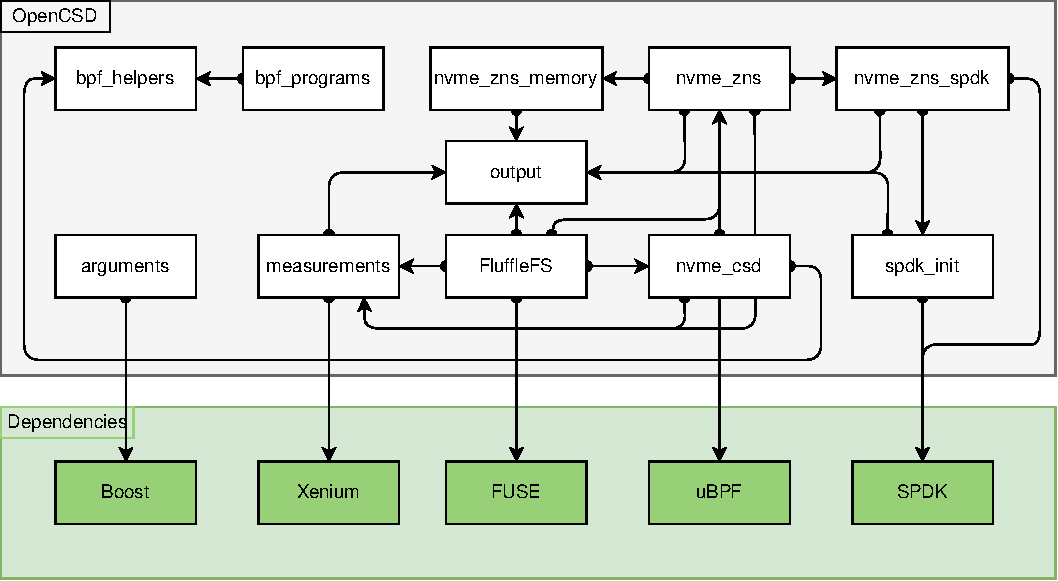
\includegraphics[width=1\textwidth]{resources/images/module-dependencies.pdf}
	\caption{Overview of all OpenCSD components and their depends-on relations}
    % \includesvg[width=0.6\columnwidth]{resources/images/module-dependencies}
    \label{figure:moduledependencies}
\end{figure}

\section{Filesystem}

% Two write pointers, one for RANDOM ZONE and one for LOG ZONE. Use of ZNS is
% optional but allows for lower write-amplification and more explicit garbage
% collection

\subsection{Concurrency}

\section{Offloading}

% Filesystem extended attributes, PID + INODE

\section{Design for Manufacter}

% Describe how the design would change for a real world, practical
% implementation. Take the ICD loader diagram as base.

% ---------------------------------------------------------------------------
% ----------------------- end of thesis sub-document ------------------------
% ---------------------------------------------------------------------------

% this file is called up by thesis.tex
% content in this file will be fed into the main document

\chapter{Implementation} % top level followed by section, subsection


% ----------------------- paths to graphics ------------------------

% change according to folder and file names
\ifpdf
    \graphicspath{{7/figures/PNG/}{7/figures/PDF/}{7/figures/}}
\else
    \graphicspath{{7/figures/EPS/}{7/figures/}}
\fi

\section{Framework}

In this section we describe the tools and techniques used with the OpenCSD
framework, detail modules and functionality and show the external dependencies
as well as internal relationships.

Firstly, OpenCSD consist of many external dependencies, most prominently
\textit{Storage Performance Development Kit} (SPDK) \cite{spdk} and uBPF
\cite{ubpf}. To reduce the barrier to entree and simplify ease of use OpenCSD
installs the majority of external dependencies in a local isolated build
directory. Subsequently, these dependencies are made available through an
environment file which configures variables such as \textit{PATH} and
\textit{LD\_LIBRARY\_PATH}. In addition, OpenCSD offers a QEMU installation and
accompanying qcow image to emulate a ZNS SSDs due to the limited availability of
these SSDs currently. However, the use of QEMU is entirely optional. Finally,
CMake \cite{cmake} is used to orchestrate the installation of dependencies and
binary targets. Due to limitations it is advised to rerun CMake after each make
command, as this prevents unnecessary recompilation of external
dependencies\footnotemark[9].

\footnotetext[9]{Due to limitations in the evaluation of file presence
conditions which are not reevaluated when executing the generated makefile.}

As said OpenCSD is comprised of modules using a component architecture.
Additionally, Each module is compiled as a static or shared library to reduce
coupling. This creates an explicit nature of exchanging information between
linked libraries that allows to identify feasibility problems at an early stage.
This is opposed to potentially only identifying such issues when creating a
first prototype. A trivial example of such infeasibilities would be using shared
memory mutexes to synchronize filesystem and CSx program behaviour.

\subsection{Modules}

The overall modules of OpenCSD are shown in figure
\ref{figure:moduledependencies} along with any external or internal
dependencies. In addition, we briefly describe the functionality of each module.
Finally, at the end of this subsection we describe the three most prominent
modules of OpenCSd.

% Diagram with overview of different modules and their used as well as
% relationships. Also show integration of open-source technologies.

\begin{figure}
    \centering
	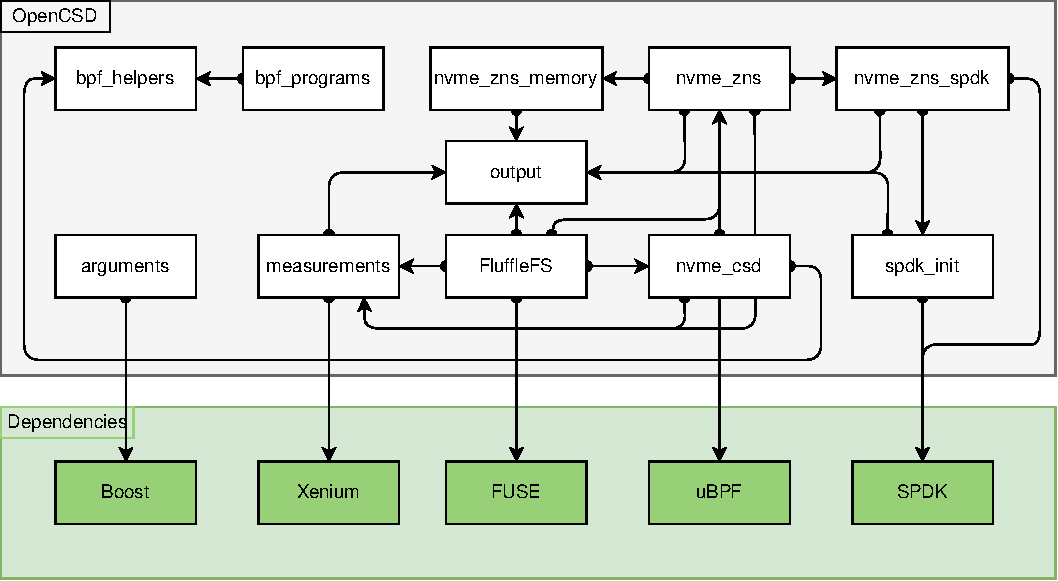
\includegraphics[width=1\textwidth]{resources/images/module-dependencies.pdf}
	\caption{Overview of all OpenCSD components and their depends-on relations}
    % \includesvg[width=0.6\columnwidth]{resources/images/module-dependencies}
    \label{figure:moduledependencies}
\end{figure}

\begin{itemize}
    \item output - Manages stdout and stderr output to the console by
    registering namespaces and providing a variety of log levels.
    \item arguments - Parses command line arguments and splits these into parts
    that can be passed to other modules in a decoupled nature. 
    \item measurements - Low overhead performance instrumentation for functions
    separated by namespaces using high performance lockless unbounded queue
    \cite{Michael1996SimpleFA}.
    \item spdk\_init - Collection of helpers to perform SPDK initialization and
    select ZNS suppporting NVMe namespace.
    \item nvme\_zns - NVMe interface to perform ZNS operations read, write and
    reset. To be used by FluffleFS for decoupled I/O operations.
    \item nvme\_zns\_memory - Memory backed implementation of nvme\_zns
    interface.
    \item nvme\_zns\_spdk - SPDK backed implementation of nvme\_zns interface
    \item nvme\_csd - Simulated extension to the PCIe NVMe protocol that allows
    to perform CSx operations. Execution of kernels is handled through uBPF.
    Utilizes instance of nvme\_zns to perform actual I/O operations performed by
    kernel.
    \item bpf\_helpers - Collection of headers that define the eBPF
    \textit{Application Binary Interface} (ABI) supported for CSx
    \textit{kernel}s. ABI to be implemented by device vendor or in this
    case nvme\_csd for simulation. The ABI is filesystem agnostic.
    \item bpf\_programs - Collection of eBPF programs linked at runtime for
    previous ZCSD \cite{lukken2021zcsd} prototype.
    \item FluffleFs - FUSE LFS supporting in-memory snapshots to achieve
    multi-user tenancy with concurrent regular and offloaded filesystem access.
    Utilizes, nvme\_zns and nvme\_csd to achieve functionality.
\end{itemize}

Out of these components nvme\_csd, bpf\_helpers and FluffleFS are the most
essential. They simulate the required changes that would be required to
realize the architecture as proposed in our simulation framework. The details of
such a practical architecture will be described later.

In short nvme\_csd contains functions that should be made part of a new NVMe
command set and namespace \cite{nvme-command} similar to how ZNS was introduced.
The functions are overly simplified so there is no use of the actual command
layout as well as lack of queue submissions and completion commands. We feel
the concepts of implementing these are well understood and would not contribute
to the scientific value of this work while introducing substantial additional
complexity.

bpf\_helpers contains the ABI exposed to the eBPF kernels. An ABI is different
from an API in that the functions it defines cannot be found in segments of
code, either included statically or through a shared library. Instead it uses
an ISA specific instruction that can be called with a set of arguments, the
arguments matching the function signature. Alternatively, should the ISA not
have a specific \textit{call} instruction, interrupt requests can be used to
achieve the same functionality. Upon calling the control flow is returned to
the operating system or in our case uBPF where the functions behavior is
implemented. The result is that an ABI allows to define functionality with
vendor agnostic implementations, similar to POSIX for operating systems. It
should be noted that ISAs typically have a hard limit on the number of arguments
that can be supported, in the case of eBPF this is five arguments.

Lastly, is FluffleFS which is described in the next separate section in detail.

\section{Filesystem}

% Two write pointers, one for RANDOM ZONE and one for LOG ZONE. Use of ZNS is
% optional but allows for lower write-amplification and more explicit garbage
% collection

\subsection{Concurrency}

\section{Offloading}

% Filesystem extended attributes, PID + INODE

% ---------------------------------------------------------------------------
% ----------------------- end of thesis sub-document ------------------------
% ---------------------------------------------------------------------------

\chapter{Consideration}

While currently both OpenCSD and FluffleFS are complete enough to performance
experimental evaluation several aspects have to be considered that can be
substantially improved. Throughout this sections those aspects are divided into
five categories. Firstly, several limitations in FluffleFS prevent regular use
of the filesystem outside of experimental settings. Secondly, the current
prototype has limited concurrency due to the use locks. Third, this simulation
framework can not be used as practical implementation and we would like to
address the necessary changes. Fourth, as previously mentioned, event kernels
suffer from unnecessary latency and data movement due to waiting for the
outstanding I/O request to complete before the kernel is submitted. To address
this we propose a mechanism for event kernels that allows the regular I/O
request to complete on the device itself. Lastly, we describe several
instruments that can be used for safety regarding user submitted kernels.

\section{Filesystem Limitations}

Firstly, the current filesystem limitations of FluffleFS make it unuseable
outside of experimental applications. Foremost, many of the datastructures are
not routinely flushed to the drive even if \textit{fsync} is called. Among
these datastructures are checkpoints, NAT and SIT blocks as well as some others.
As a result, the filesystem is incapable of restoring the previous state when
remounting a previously created filesystem.

Beyond basic setup and teardown is the inability to perform garbage collection.
Meaning no used drive space can be reclaimed. This prevents FluffleFS from
reaching steady state. The ability to delete files and directories is also
currently missing.

Lastly, since several datastructures are not flushed to the drive some mechanism
to read data from the drive are not in place. For instance \textit{lookup} will
never traverse the \textit{inode\_lba\_map} and instead solely relies on
\textit{path\_inode\_map}. This results in the \textit{path\_inode\_map} not
being used for caching instead containing all paths from all to all files and
directories for the entire fileystem.

While it is important to clearly describe the severe practical shortcomings of
FluffleFS note that all these limitations are resolved in the design. Given the
requirements set out by the experiments and time constraints implementing these
features is left as future work.

\section{Concurrency}

Similarly, the degree of concurrency achieved throughout OpenCSD and FluffleFS
is significantly less then possible with the current design. Both time
constraints and these optimizations not being required for the experiments have
led to the decision to prioritize elsewhere. This section describes several
areas that can easily be improved.

Firstly, every filesystem operation utilizes a global lock. As mentioned
previously this MRSW lock allows some operations to operate concurrently while
providing mutual exclusion for critical operations. However, many of the
operations currently utilize the lock in the mutually exclusive mode (writer)
while this can be avoided if underlying datastructures are better protected.
These include in no particular order \textit{lookup}, \textit{getattr},
\textit{setattr}, \textit{readdir}, \textit{open}, \textit{release},
\textit{create}, \textit{fsync}, \textit{getxattr} and \textit{setxattr}.

With such a predominant amount of the operations being entirely serialized with
respect to one another it is very likely this will hinder performance in a
non-neglible manner. For completeness, the remaining operations include
\textit{read} and \textit{write} as necessary per our design requirements to
achieve concurrent regular and offloaded access.

Beyond the filesystem itself the current NVMe backend also suffers from limited
concurrency. In a similar manner this is due to the use of a global lock that
serializes the incoming \textit{read}, \textit{append} and \textit{reset}
operations together. This current limitation is necessary as currently a single
SPDK queue of 4096 bytes in size is used. However, both SPDK and the underlying
NVMe device are capable of having multiple operations being queued concurrently.
While several limitations apply such as only one pending \textit{append} per
zone\footnotemark[16] it is clear a lot of the underlying drive performance is
unutilized in this manner.

\footnotetext[16]{Although multiple sectors can be written in this single
append, within ZNS this is known as queue depth beyond one.}

Importantly, utilizing multiple pending operations is not the same as supporting
an iodepth beyond one neither is it utilizing ZNS append with a queue depth
beyond one.

Last is UBPF as the current system for scheduling kernels can only support one
instance concurrently. Because of this all calls to start running a new kernel
are serialized using a global lock. This last problem is less trivial to resolve
compared to those previously discussed. Within uBPF an instance of the VM object
needs to be bound to methods as key value pairs. Here each key is a specific
number that is supplied as first argument to the \textit{call} instruction in
the eBPF ISA. However, the signature of these hooked methods is identical as how
it will be exposed to the eBPF kernel. This leaves no state or arguments that
can be passed along to associate the specific instance of uBPF once trapped into
the hooked method.

% Figure of transition between kernel and host with method signature and how
% this can't be associated to correct instance (show 3 as example).

A possible solution would be to pass the instance of uBPF as first argument and
supplying the kernels with the instance of their own VM. This breaks isolation
and has many negative side effects in terms of security as well requiring the
disabling of the memory access verifier.

Instead, each instance of uBPF should be associated with a unique sufficiently
sized hash that is presented to the kernel instead. Upon each \textit{call} this
hash is passed as first argument. Once trapped inside the method this hash is
looked up and matched to its respective instance. Should there be no matching
hash the kernel will immediately be terminated. Given a sufficiently large
hash domain the change of a malicious actor finding a match for any concurrently
running instance of uBPF that is not its own are net zero.

% figure of transistion between kernel and host with hash as first argument and
% reverse lookup inside hash table to find uBPF instance.

Clearly, there are many potential performance improvements related to
concurrency that could benefit the current OpenCSD and FluffleFS prototype.

\section{Design for Manufacter}

Beyond concurrency the current prototype suffers from several design decisions
and implementations details that are not suitable for pracitcal implementations.
Many of these limitations arise from being a monolithic application simulation
the offloading rather than submitting it to an actual embedded device. In this
section the necessary changes to create real world practical implementations are
described.

Firstly, the current proposed changes to the NVMe command set are implemented as
shared library linked at compile time. Such an interface where data can be
easily moved back and forth is not pracitcal for systems utilizing communication
protocols and busses. This interface needs to be redesigned with limitations of
these protocols inmind such as limited request size of individual commands and
the asynchronous nature of command submissions. Luckily many extensions to
the NVMe protocol already exist, ZNS being a notable example.

Secondly, the interface exposed to user submitted eBPF kernels needs to be
formalized. Furtermore, this interface needs to be ratified as part of the NVMe
protocol extension so that the minimum set of supported calls from within 
user submitted kernels is non-optional. This will prevent users from having to
rewrite or recompile kernels across different vendors. Given the limited compute
capabilities typically found on these embedded platforms runtime evaluation of
appropriate interfaces should not be an acceptable solution either.

Third, once the new extension to the NVMe command set is ratified existing
drivers such as SPDK, xNVME or those found in the Linux kernel need to be
updated to support this. Likely both the driver and the firmware on the device
will be responsible for scheduling of submitted kernels. Some ideas on this are
detailed while discussing \textit{filesystem agnostic kernels} but no complete
scheduling solution is presented in this work.

Finally, we show an example of the complete data path across all components as
described in this section in figure \ref{figure:practicalarchitecture}.

\begin{figure}
    \centering
	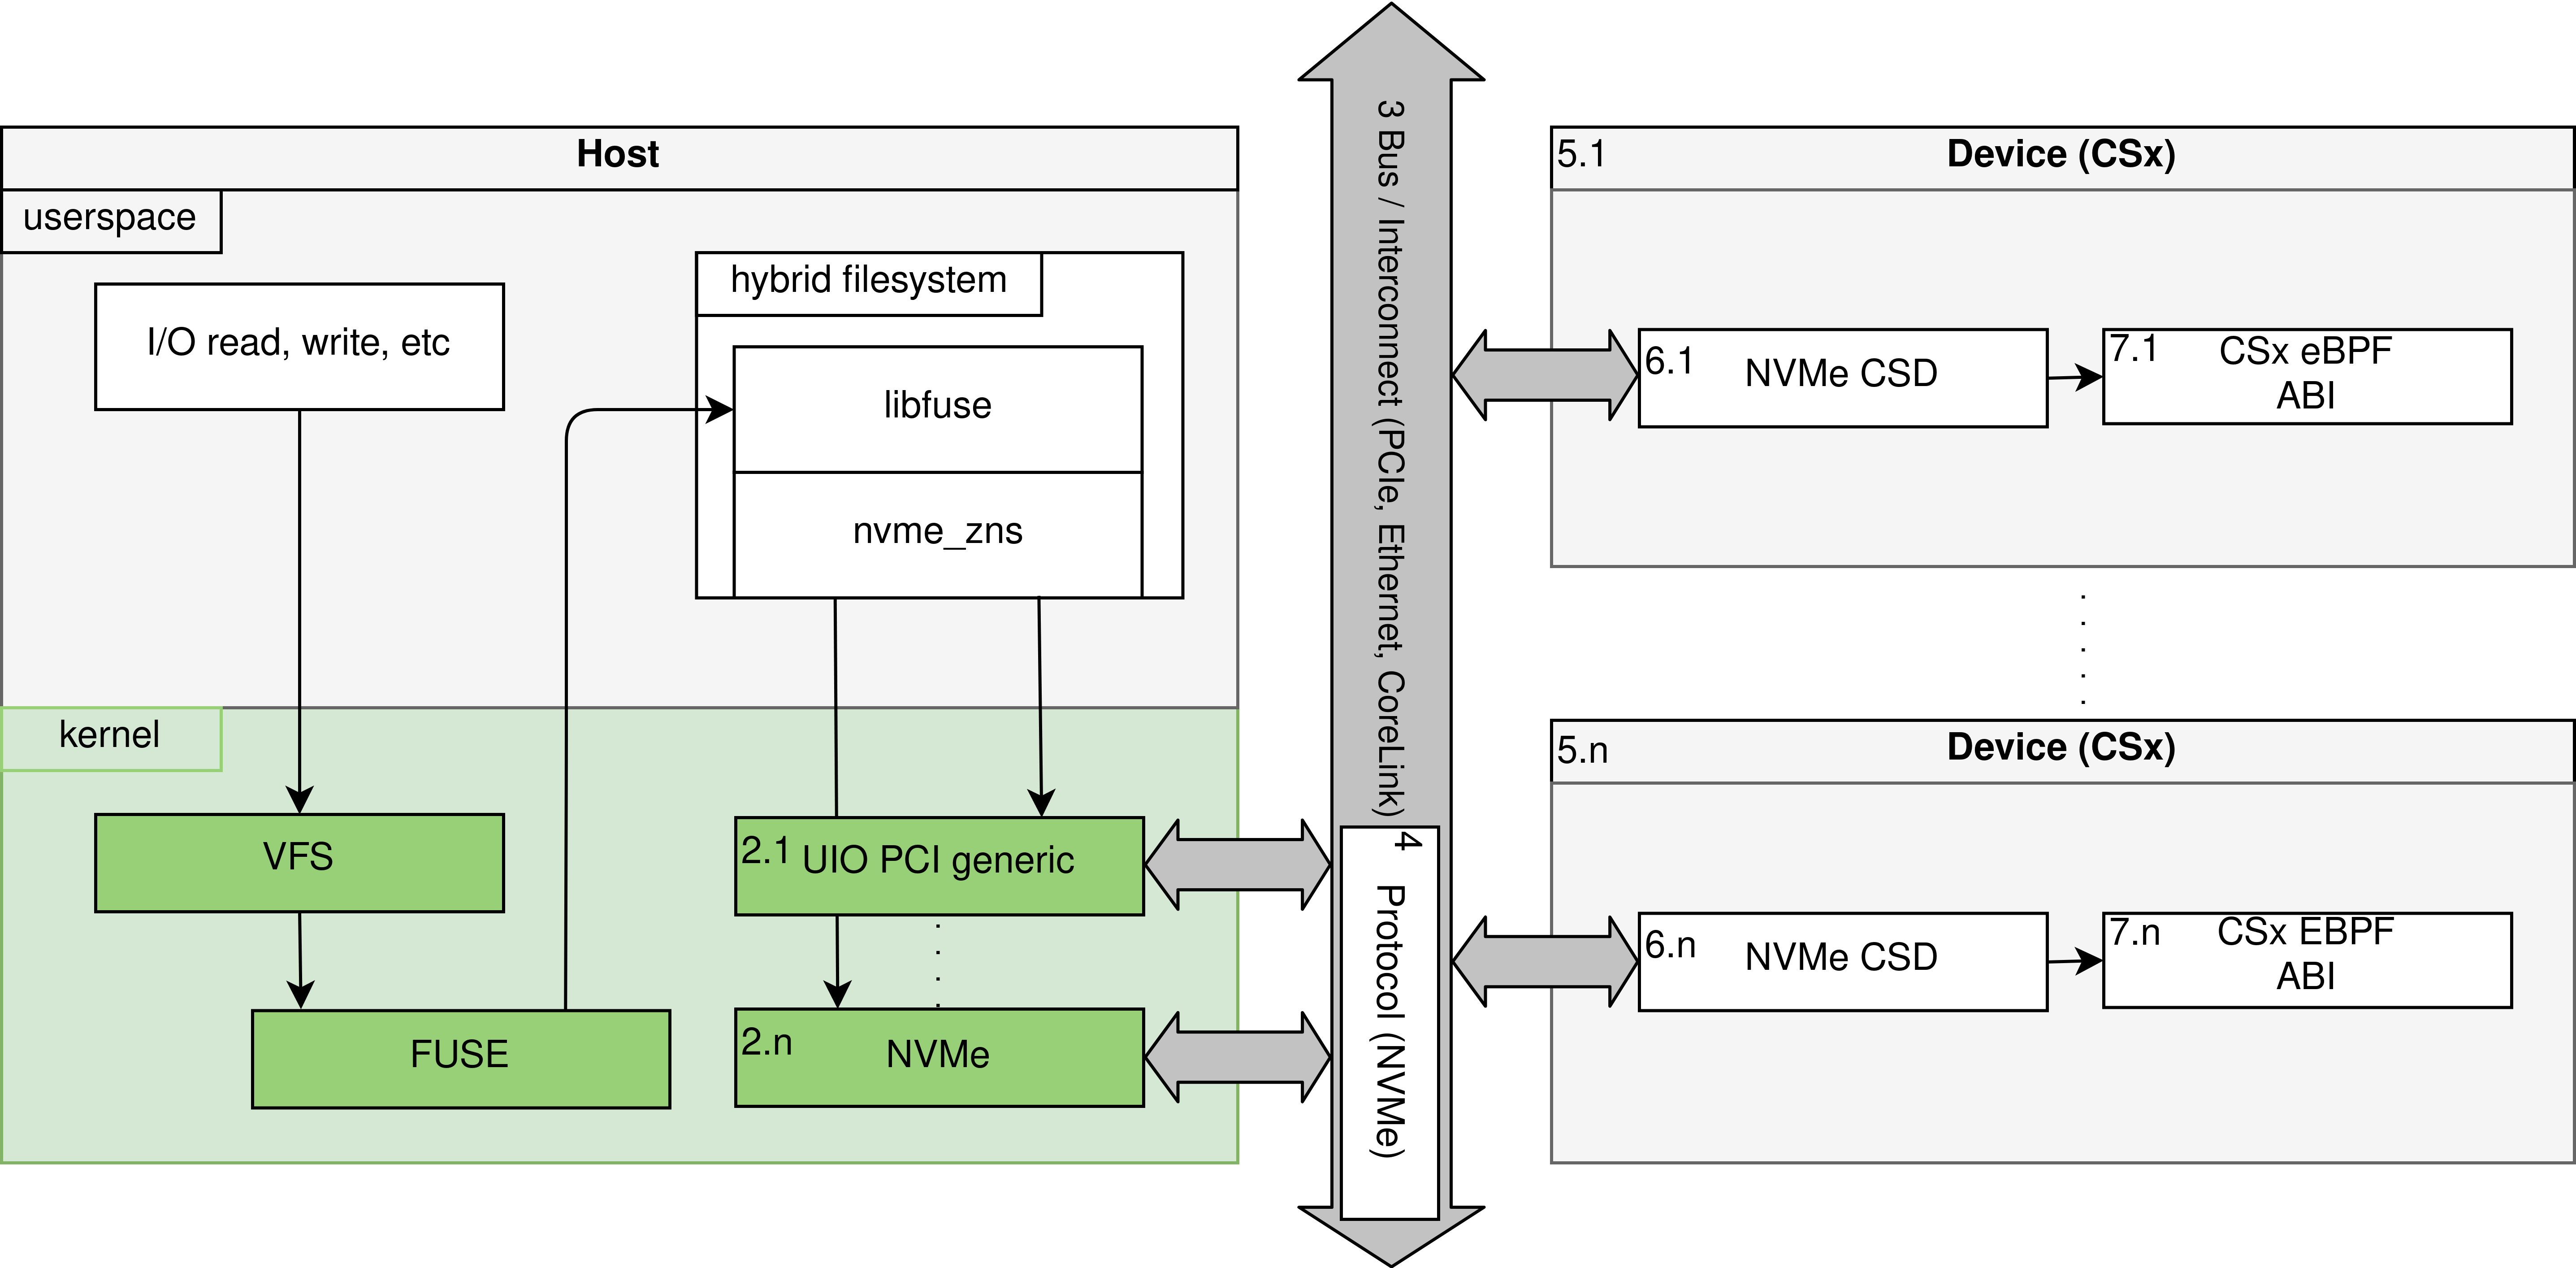
\includegraphics[width=1\textwidth]{resources/images/loader-pfs-arch-v3.png}
	\caption{Practical complete architecture for vendor agnostic CSxs with
        potential filesystem support.}
    % \includesvg[width=0.6\columnwidth]{resources/images/module-dependencies}
    \label{figure:practicalarchitecture}
\end{figure}

\section{Effective Event Kernels}

As mentioned the current event kernel implemenation suffers from unnecessary
data movement and latency. To demonstrate this situation the data path across
requests to and from the CSx is shown in figure
\ref{figure:currenteventkernels}. In this figure the process of opening the file
and setting the extended attribute has been omitted.

\begin{figure}
    \centering
	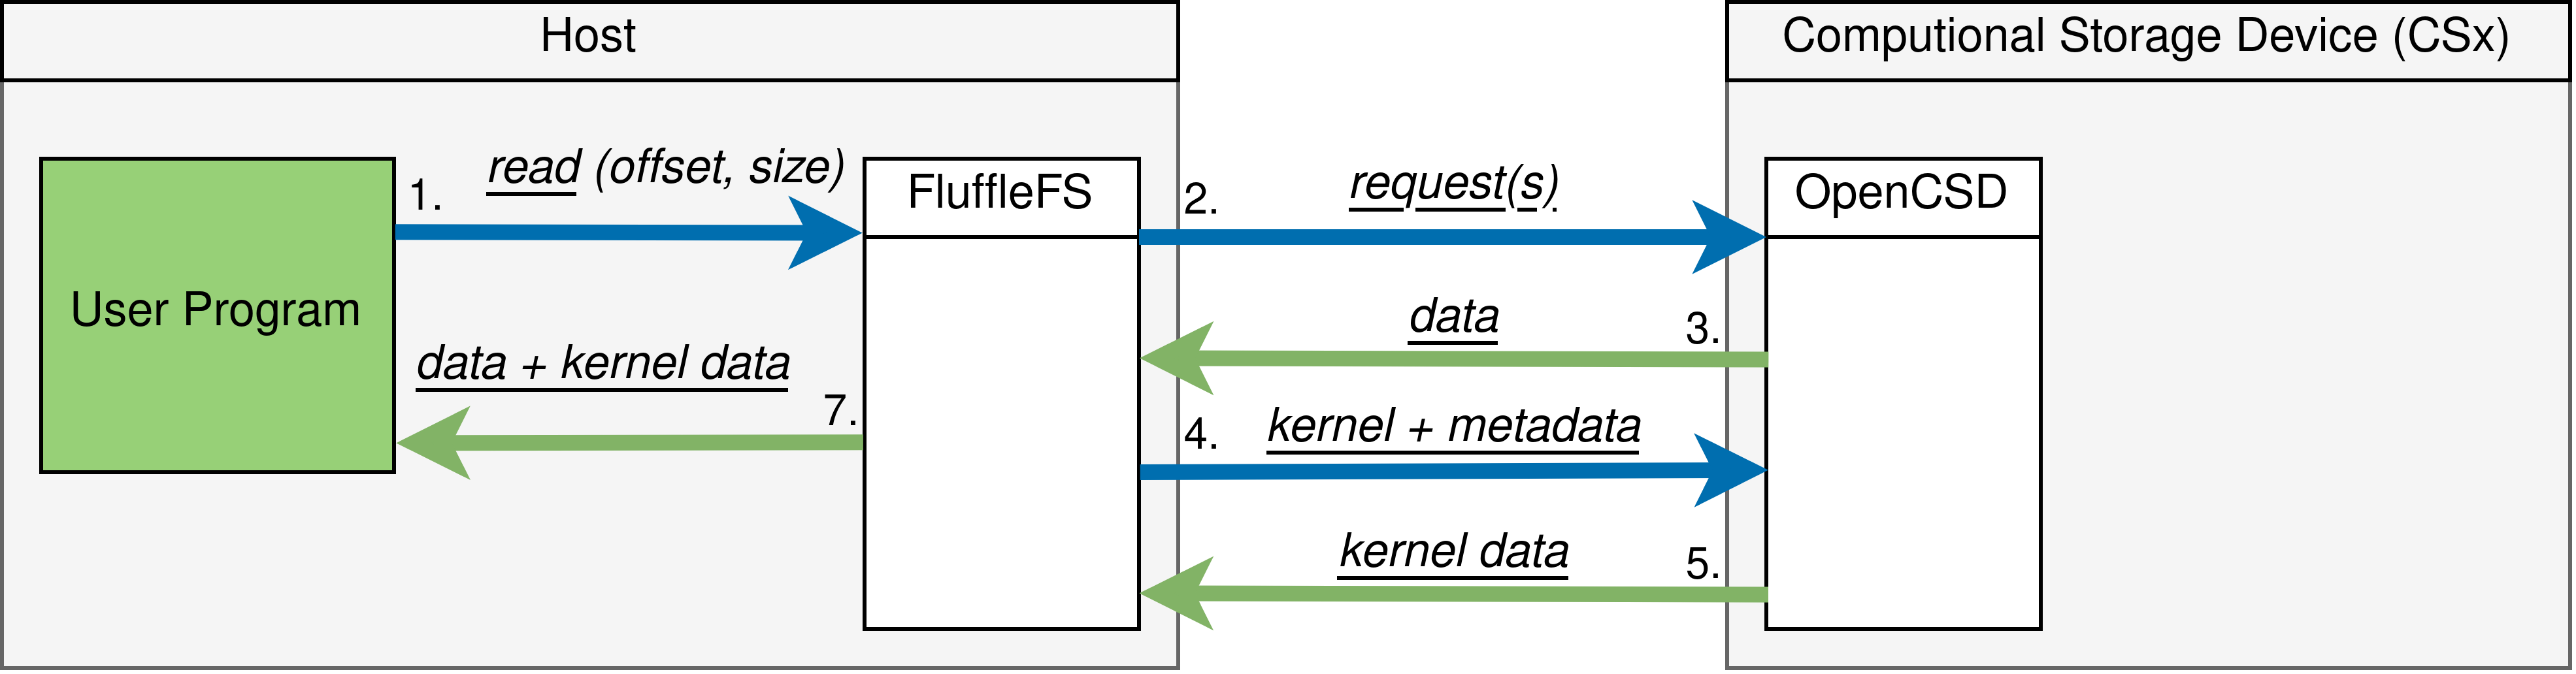
\includegraphics[width=1\textwidth]{resources/images/current-event-kernel.png}
	\caption{Current implementation of event kernels.}
    % \includesvg[width=0.6\columnwidth]{resources/images/module-dependencies}
    \label{figure:currenteventkernels}
\end{figure}

As shown the filesystem sends the request along to the drive after receiving the
read request from the user. After receiving this data in step three the
filesystem can now submit the user kernel along with the necessary metadata to
the CSx. Finally, after the kernels completion the combined data can be returned
to the user. The procedure is identical for write requests except no data is
returned to the host upon completion of the request and the kernel.

In order to reduce the latency and unnecessary data movement we propose a
multistage kernel mechanism consisting of five steps.

\begin{enumerate}
    \item The filesystem submits a kernel to perform the relative read or write
    request as normally performed by the filesystem from the host side. Such
    a kernel operation is known as \textit{passthrough}. The return data of this
    kernel is the necessary metadata that needs to be provided to the user
    submitted kernel.
    \item The user submitted kernel is presented with the metadata from the
    first kernel and starts executing normally.
    \item Along the return data from the user submitted kernel metadata is
    provided as monitored by the CSx. This metadata reports written and read
    sectors.
    \item The filesystem verifies that the return data from the user submitted
    kernel matches the reported metadata. For instance, the file size from a
    write event kernel can not increase by two sectors if only one sector
    was written.
    \item The filesystem modifies the datastructures related to the file if
    necessary.
\end{enumerate}

The five steps create a solution that prevents unnecessary data movement and
reduces latency but does not clearly address several safety concerns regarding
malicious user submitted kernels. Among this is the non-trivial task of
verification. To alleviate this we propose that event kernels should only be
able to append data to the end of a file. Under these circumstances the user
submitted kernel can not send malicious metadata that would indicate other parts
then those intended of the file had actually been rewritten. In addition, this
prevents significant additional complexity from otherwise merging the new
data in between the existing parts of a file.

Among event kernels are several other safety concerns as laid out in our
research question but these will be addressed separately in the last section of
the consideration.

\section{Filesystem Agnostic Kernels}

The current prototype is carefully designed to allow users to write programs
once and reuse it across vendors. For this we have created a specific header
supporting various calls as explained in the implemenation section.
Unfortanetely, however, to synchronize these kernels with the filesystem
additional datastructures and calls are needed. For know these have been defined
in a header specific to FluffleFS. In this section we describe a mechanism for
many computational storage filesystems to have their own specific behavior and
mechanism but still allow for agnostic user kernels when offloading.

At the core of these filesystem agnostic kernels is the CSx filesystem runtime.
We show it and all its various components in figure \ref{figure:csxfsruntime}.

\begin{figure}[H]
    \centering
	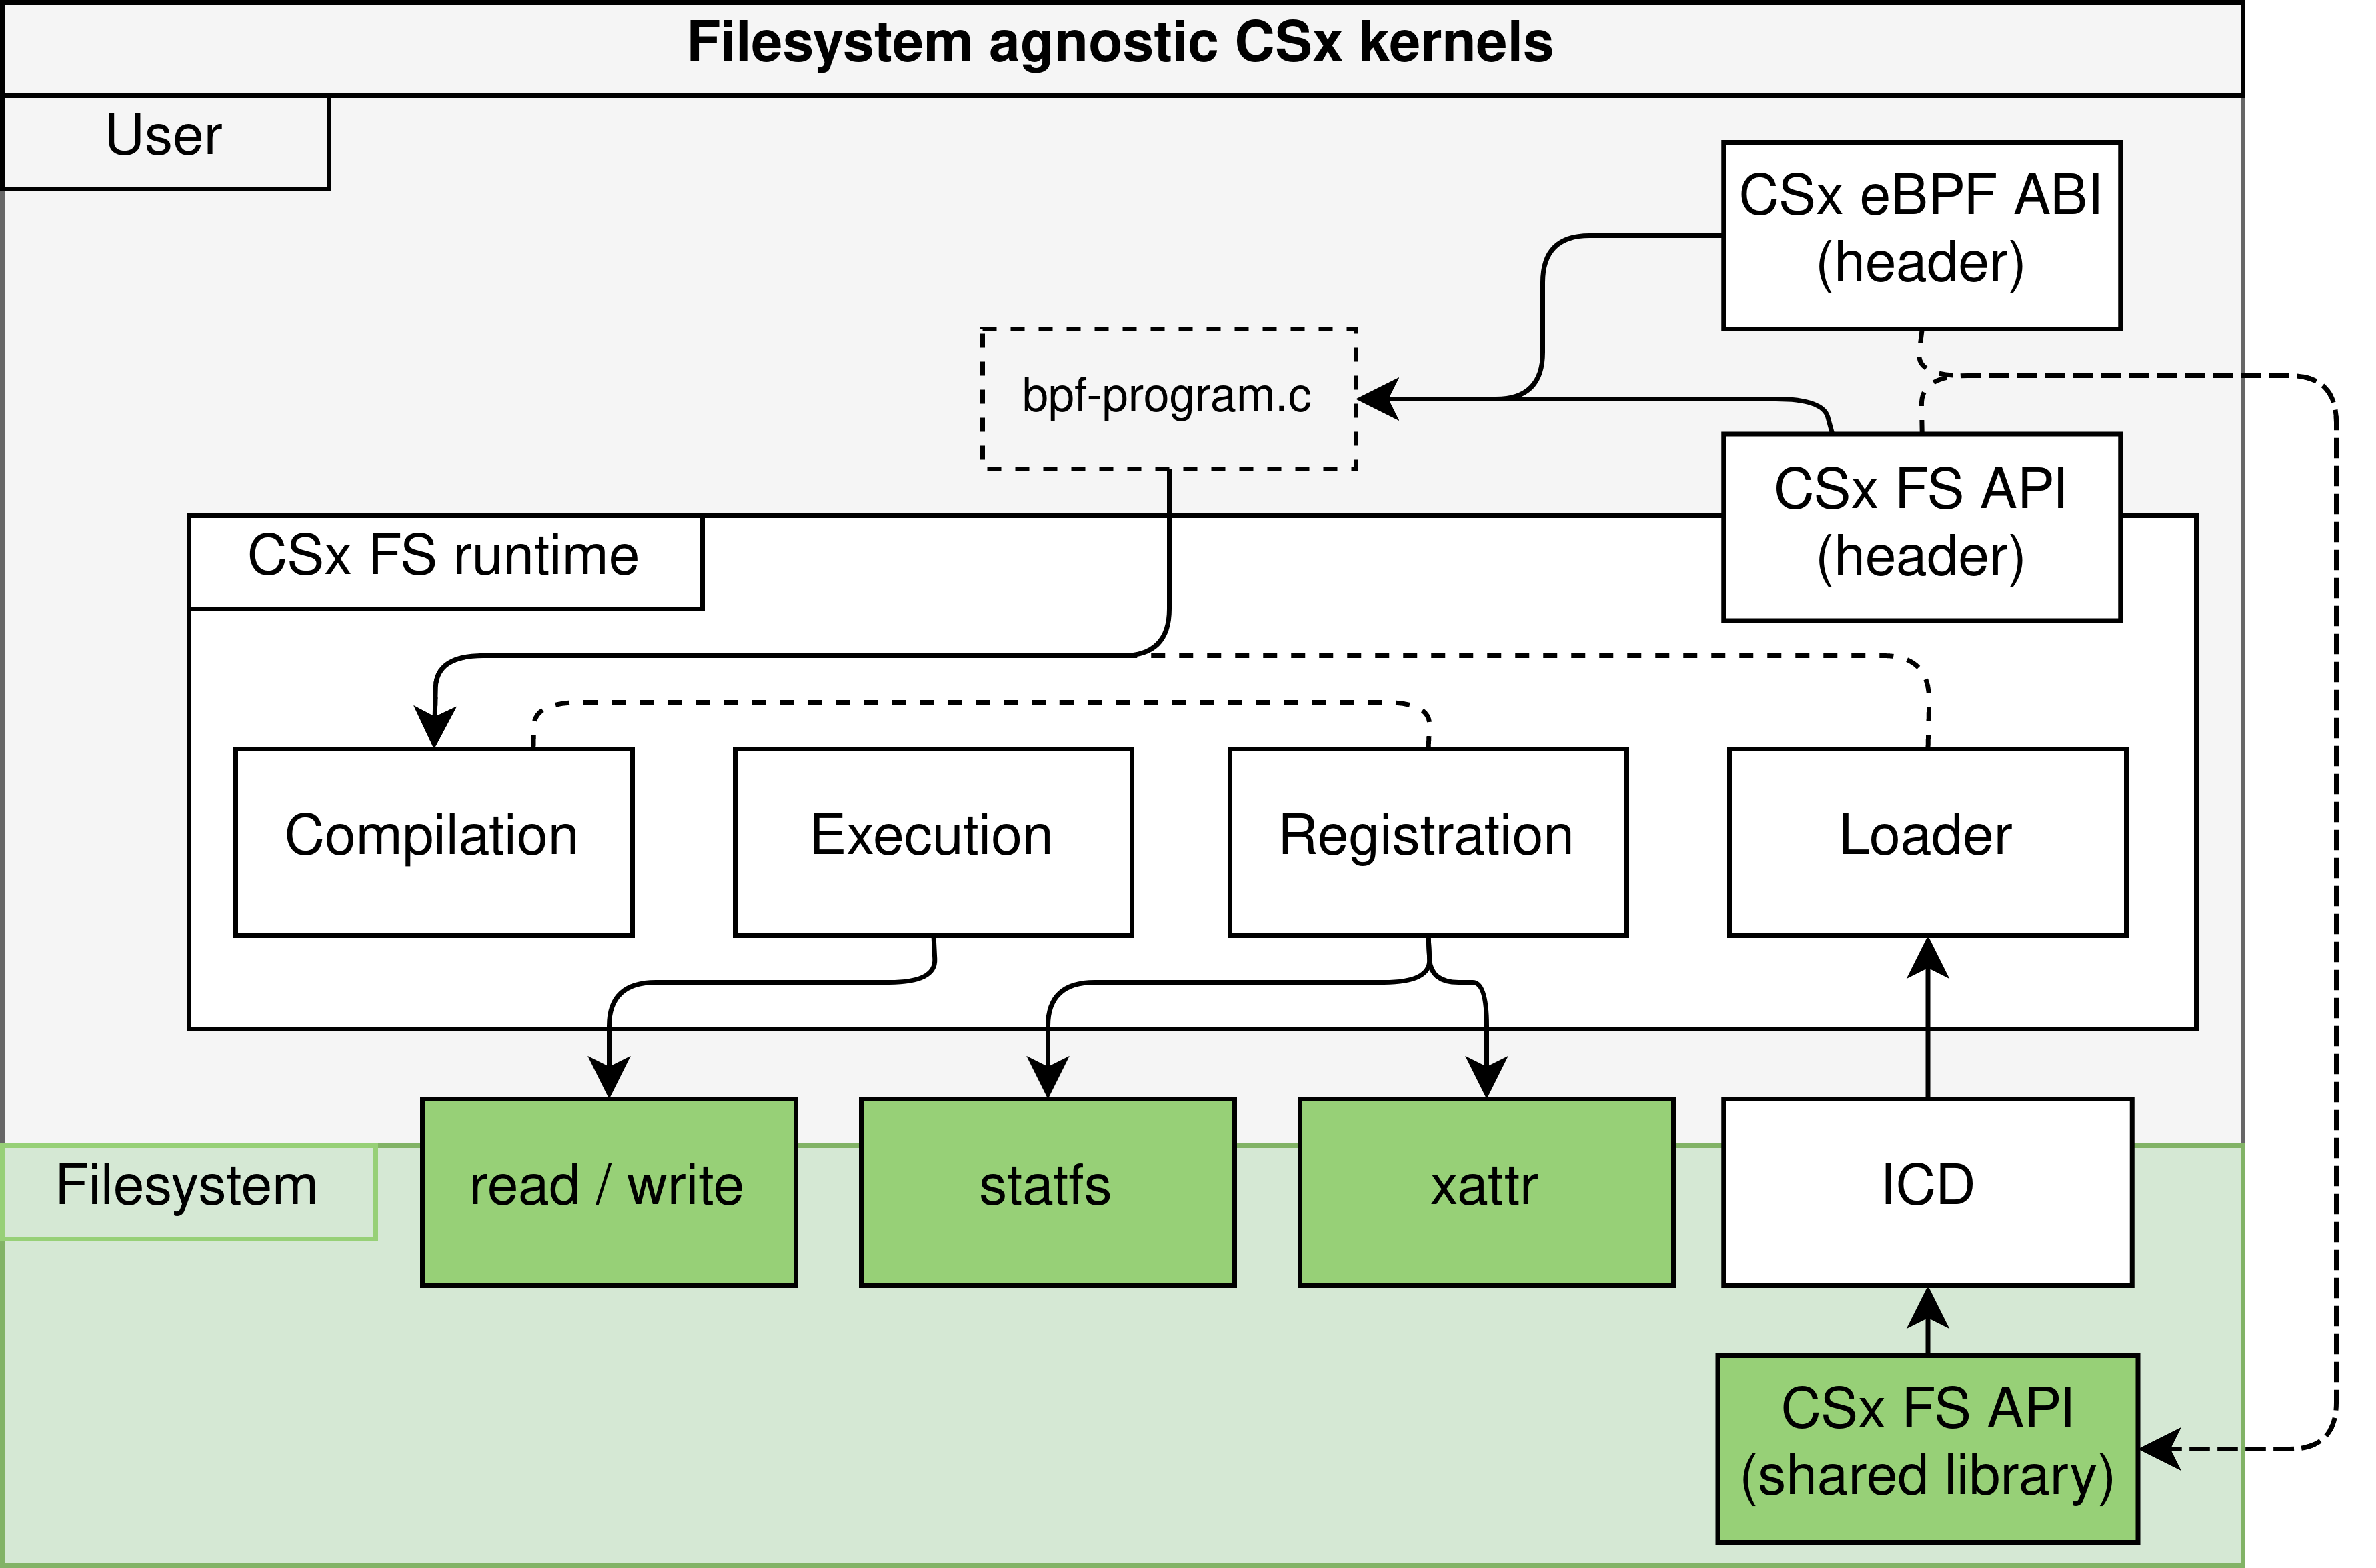
\includegraphics[width=0.7\textwidth]{resources/images/csx-fs-agnostic.png}
	\caption{Extended architecture to support filesystem agnostic CSx kernels.}
    % \includesvg[width=0.6\columnwidth]{resources/images/module-dependencies}
    \label{figure:csxfsruntime}
\end{figure}

Through this runtime the filesystem specific implementation of several
filesystem operations will be supplied. The required set of operations and
datastructures needs to be formalized and made part of the extension to NVMe
command set. Through the dynamic loading of shared libraries using a technique
from graphics APIs called \textit{Installable Client Drivers} (ICDs) the user
will not have to deal with recompilation. Such an ICD contains additional
metadata in a human readable markup language and can support extensions. The
CSx runtime can identify the filesystem and ICD for the current offloaded
operation through the use of \textit{statfs}. Furthermore, such a runtime can
provide host side scheduling mechanisms that are likely necessary in performant
multi-user tenancy applications.

% Use statfs to determine the type of filesystem, ICDs are related to a specific
% filesystem type. The CSx eBPF ABI should contain atleast one system call to
% retrieve the vendor filesystem context data for the current request (already
% part of prototype). The CSx FS API contains functions and datastructures to
% allow the kernel to transform this context data. The API is implemented by
% individual filesystems as shared library and made available throught the ICD.
% The CSx FS runtime uses a loader with mechanisms such as \textit{dlopen} to
% verify the contents of the provided library in accordance to the API.

% The basic format of the ICD can be extended such that it could support
% extensions to the base API as well as contain versioning. Typically, ICD files
% are human readable using a markup language such as YAML. This is same approach
% as the prominent video graphics API Vulkan.

\section{Kernel Safety}

The last consideration proposes mechanisms to ensure the execution of user
submitted code occurs safely. In the context of a filesystem this includes
preventing modifications to other files or regions of files. Additionally, it
requires preventing that an user submitted kernels reads regions of files it
should not have access to. Commonly the so called \textit{security triad} is
used to categories the different aspects of security. These
include confidentiality, integrity and availability. Confidentiality ensures
that no one is able to access data they should not be able to while integrity
ensures any data that is read is not modified by an attacker. Lastly,
availability needs to ensure the system remains operational even in the face of
an attack.

A potential first line of defence is the same system used by the Linux kernel
namely, static verification. Through static verification the Linux kernel
determines the behavior of an user submitted kernel prior to its execution.
However, to be able to determine the entire behavior statically many limitations
on how the kernel can be written need to be imposed. Particularly, loops with
bounds determined by parameters are problematic. This is because not only
false reporting of metadata, writes attributes to other files but also
termination can cause issues. A malicious user submitted kernel could
intentionally run an infinite loop, never terminating and consuming system
resources. To implement such a static verification system for eBPF existing
open-source tools such as ebpf-verifer \cite{ebpf-verifier} can be used.

Beyond static analysis the CSx can record metadata and instrumentation that
reports about the behavior the kernel exhibited. Since each time an operation of
the ABI is called the uBPF VM traps into vendor code there would be no effective
mechanism for the user submitted kernel to hide this activity. Potentially, the
CSx could even immediatelly terminate the user submitted kernel without
executing the requested operation entirely. For example, the regions of a file
is supposed to read need to be provided with metadata upon kernel submission.
By formalizing the structure of this metadata the vendor will be able to analyze
it as well. Consequently should any ABI call be made to \textit{read} or
\textit{write} to a sector not defined in this metadata the kernel can be
immediately terminated. Granted the more flexible user submitted kernels become
the harder it becomes to identify malicious behavior. Luckily the currently
proposed stream and event kernels both would limit malicious behavior to a
single file. This is due to the append only nature of ZNS devices as well as the
absence of the \textit{reset} command from our ABI.

Lastly, the current implementation of uBPF can be extended such that the access
verifier can work even for JiT code. This can either be achieved by
instrumenting instructions during the jitting itself or through hardware
mechanisms in the embedded compute device. Several embedded devices already have
similar technologies such as ARM TrustZone \cite{Pinto2019DemystifyingAT}.

It is unfortunate that none of the envisioned safety mechanisms could be
implemented in the current prototype. However, the restrictive nature of the
current stream and event kernels still make execution relatively safe. For a
user to submit a kernel to operate on a target file it must have access to this
file as determined by the filesystem \textit{Access Level Control} (ACL).
Should the user not have access the kernel will not be submitted. As described,
both kernels are only able to modify the file they operate on resulting in users
only being able to modify files they have access to.

Several important safety considerations are not captured by our prototype
however. it is still able to defend the integrity of data. Confidentiality and
availability can not be guaranteed in the current form. As examples, an user
submitted kernel can read arbitrary sectors on the drive as well as submit
kernels with infinite loops. Throughout this section sufficient mechanisms are
defined to ensure confidentiality and availability can be guaranteed as well.
By guaranteeing all three aspects of the security triad we can provide safe
user submitted kernels.

% ---------------------------------------------------------------------------
% ----------------------- end of thesis sub-document ------------------------
% ---------------------------------------------------------------------------

% this file is called up by thesis.tex
% content in this file will be fed into the main document

\chapter{Experiments} % top level followed by section, subsection


% ----------------------- paths to graphics ------------------------

% change according to folder and file names
\ifpdf
    \graphicspath{{7/figures/PNG/}{7/figures/PDF/}{7/figures/}}
\else
    \graphicspath{{7/figures/EPS/}{7/figures/}}
\fi


% ----------------------- contents from here ------------------------
% 

\section{Experiment Design}

In this section we designed several experiments to evaluate the performance of
FluffleFS. These experiments can be separated into two categories. Firstly,
we performed microbenchmarks operating on relatively simple reads and writes.
Secondly, we isolated several applications that likely benefit from offloading
and port these to be used by FluffleFS. For each of these applications we reason
about the expected and achieved data movement reduction among other performance
metrics.

For each of the experiments measurements are taken 30 times to account for
variance between measurements. For almost all measurements the mean will
be used alongside minimum and maximum errors bars.

\subsection{Microbenchmarks}

Most of these microbenchmarks serve to compare performance against more
established ZNS supporting filesystems. For these microbenchmarks the popular
F2FS\cite{Lee2015F2FSAN} filesystem is used. Exceptions to these include
evaluating the offloading and concurrent performance of FluffleFS against its
regular performance.

E
Each of these benchmarks is executed on a freshly formatted filesystem each
time due to the inability of FluffleFS to reach \textit{Steady State}. while
F2FS is able to reach steady state a comparison between filesystems in such
substantially different states would be unfair.

\begin{enumerate}
    \item Sequential reads \& writes f2fs vs FluffleFS
    (Linegraph transfer rate MB/s - 64k up until 1g filesizes)
    (Static request size of 512k unless file is smaller)
    \begin{itemize}
        \item Demonstrate what performance can be expected from FluffleFS as
              regular filesystem.
    \end{itemize}
    \item Random reads \& writes f2fs vs FluffleFS
    (Linegraph transfer rate MB/s - 4k, 8k, 16k, 32k, 64k, 128k request sizes)
    (Static file size of 1g, this is to exhaust caches and their effects)
    \begin{itemize}
        \item Demonstrate what performance can be expected from FluffleFS as
              regular filesystem.
    \end{itemize}
    \item Sequential reads \& writes regular vs passthrough kernel
    (Linegraph transfer rate MB/s - 64k up until 1g filesizes)
    (Static request size of 512k unless file is smaller)
    \begin{itemize}
        \item Show performance impact of snapshotting and uBPF.
    \end{itemize}
    \item Sequential reads \& writes concurrently regular \& 1 passthrough 512k
    request size
    (Linegraph, 1, 2, 4, 8 threads, with best performer previous benchmark)
    \begin{itemize}
        \item Demonstrate the passthrough kernel performance is relatively
              unaffected compared to deminishing performace of regular reads
              \& writes for multiple threads. (Proof concurrent access to the
              same file).
    \end{itemize}
\end{enumerate}

\subsection{Applications}

\begin{enumerate}
    \item Offload integer average (read stream kernel)
    \begin{itemize}
        \item Have one thread write append to a file while the another computes
              the integer average for this file do so using both regular access
              and using kernel offloading.
        \item Demonstrate offloading can reduce amount of data transfered
              between host and device significantly with no signifcant
              performance impact.
    \end{itemize}
    \item Offloaded shannon entropy (read stream kernel)
    \begin{itemize}
        \item Go through all files in a directory and determine entropy of first
              512k of each file. Return a list of files with entropy < 6.
        \item Demonstrate that async applications can reduce host load by
              waiting for offloaded tasks (Total CPU time - kernel CPU time)
    \end{itemize}
    \item CSV index generation (write event kernel)
    \begin{itemize}
        \item Generate indexes for a query replicated from TPC-DS at 512k
              intervals.
        \item Demonstrate that async applications can reduce host load by
              waiting for offloaded tasks (Total CPU time - kernel CPU time)
    \end{itemize}
\end{enumerate}

\section{Experimental Setup}

% Machine host, configuration, kernel version, modules and versions,
% software compiler flags

% Use alacritty to prevent performance influence of writing to stdout / stderr


\subsection{Pitfalls}

% ---------------------------------------------------------------------------
% ----------------------- end of thesis sub-document ------------------------
% ---------------------------------------------------------------------------

\chapter{Results}

This section describes the results from the previously defined experiments.
Similar to the experiments section these results are separated into two
categories being microbenchmarks and applications.

For each result we explain the information being presented as well as further
findings. In addition, probably causes are discussed as well as
potential future experiments to investigate these claims.

\section{Microbenchmarks}

Several of the results for microbenchmarks are grouped together such as
sequential read and write results. Furthermore, all microbenchmark results use
line-graphs scaled with $log4$ on the horizontal axis. Using this scaling the
distance between different file and request sizes is proportional to their
difference in size.

\subsection{Sequential Results}

Our first results compare the sequential read and write performance of F2FS
against FluffleFS. These results are shown in figures
\ref{figure:readsequential} and \ref{figure:writesequential} respectively.
While the performance is similar for the smallest 64KiB file size each larger
filesize constitutes and increasingly larger performance gap. Notable
observations include the large difference between the minimum and
maximum write throughput in F2FS as well as a collapse in throughput for files
beyond 256MiB in size. A similar but much smaller drop can also be observed in
write throughput for FluffleFS.

\begin{figure}[h]
    \centering
	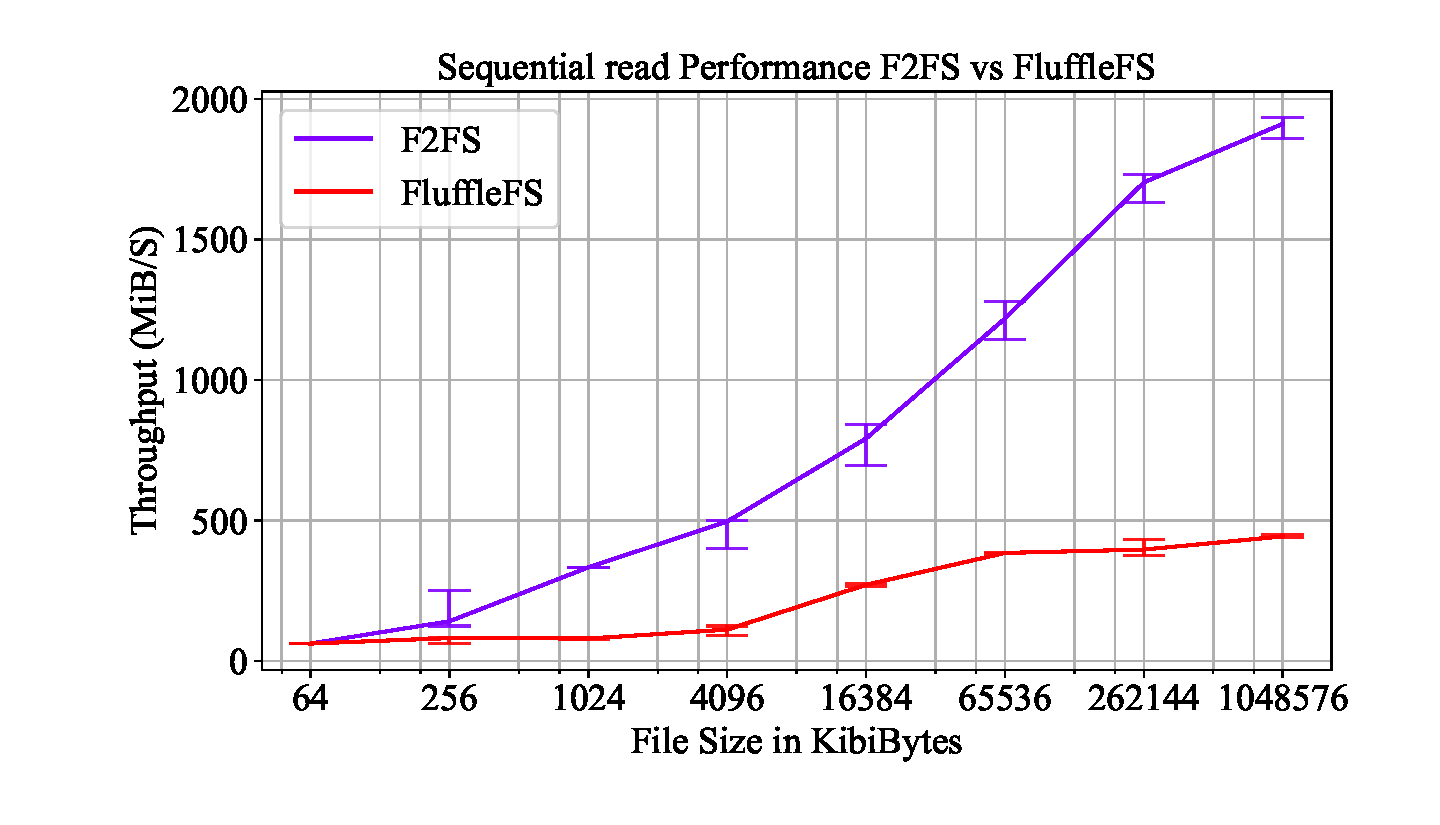
\includegraphics[width=1\textwidth]{resources/images/results-sequential.pdf}
	\caption{Results of sequential read microbenchmark evaluation using a request
        size of 524288 bytes or equal to file size if lesser.}
    % \includesvg[width=0.6\columnwidth]{resources/images/module-dependencies}
    \label{figure:readsequential}
\end{figure}

\begin{figure}[h]
    \centering
	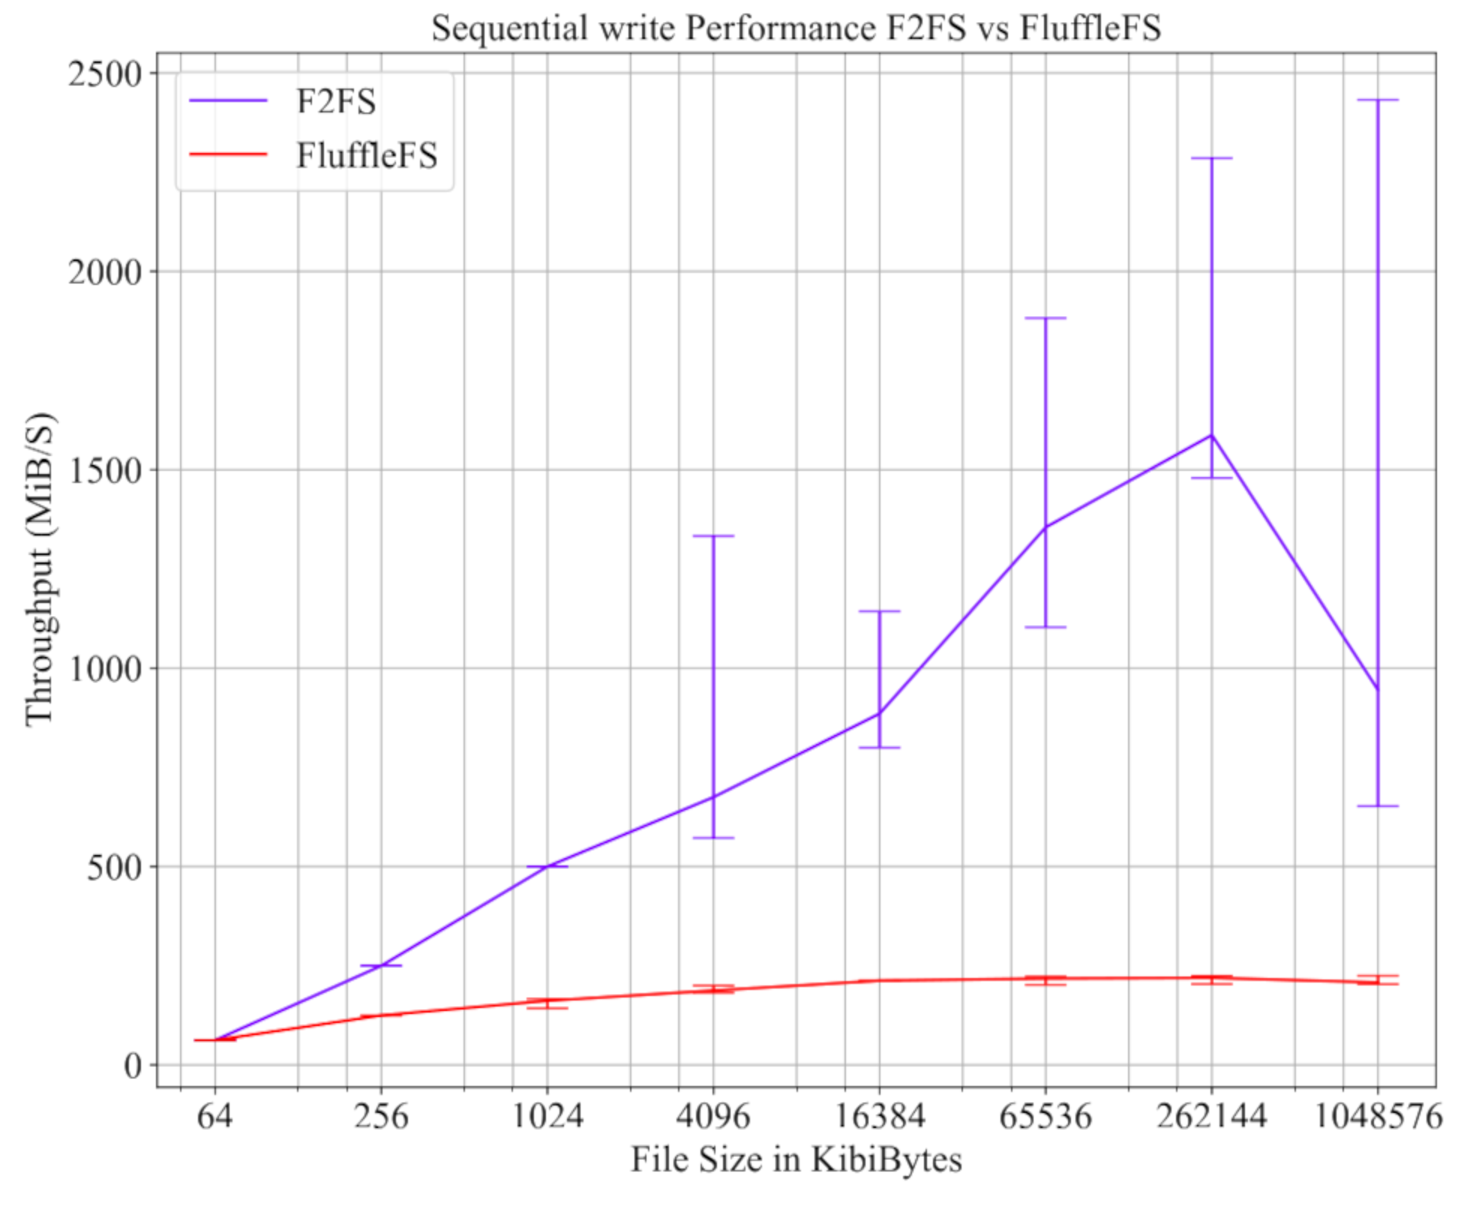
\includegraphics[width=1\textwidth]{resources/images/results-sequential-write.pdf}
	\caption{Results of sequential write microbenchmark evaluation using a request
        size of 524288 bytes or equal to file size if lesser.}
    % \includesvg[width=0.6\columnwidth]{resources/images/module-dependencies}
    \label{figure:writesequential}
\end{figure}

\subsection{Random Results}

Random read and write performance has fastly different results the most notable
is random read performance as shown in figure \ref{figure:readrandom}. Here both
F2FS and FluffleFS reach about 25\% of their previous performance for sequential
reads regarding largest file and request size respectively. Notable is that
the performance of F2FS and FluffleFS is comparable for random reads using a
request size of 4096. Coincidentally, this size is equal to the sector size of
the underlying ZNS device. Furthermore, the performance F2FS achieves for 4096
byte requests maintains roughly equal for lower request sizes. Contrarily,
FluffleFS loses considerable performance for smaller request sizes below
4096 bytes.

Several mechanisms in FluffleFS are likely the cause for this performance
discrepancy. Firstly, FluffleFS submits I/O requests rounded up to the nearest
sector size regardless of how much data it actually needs. Secondly, the
interface between FluffleFS and the NVMe backend perform unnecessary copying of
data. This interface should be updated to use zero-copy instead. Lastly,
FluffleFS allocates and deallocates buffers for each I/O request instead of
reusing previously allocated buffers. Instead FluffleFS should use a memory-pool
only allocating memory during startup and reusing it during the lifetime of the
filesystem. We believe that these are the most likely reason for the
performance difference across small request size random read operation.

\begin{figure}[h]
    \centering
	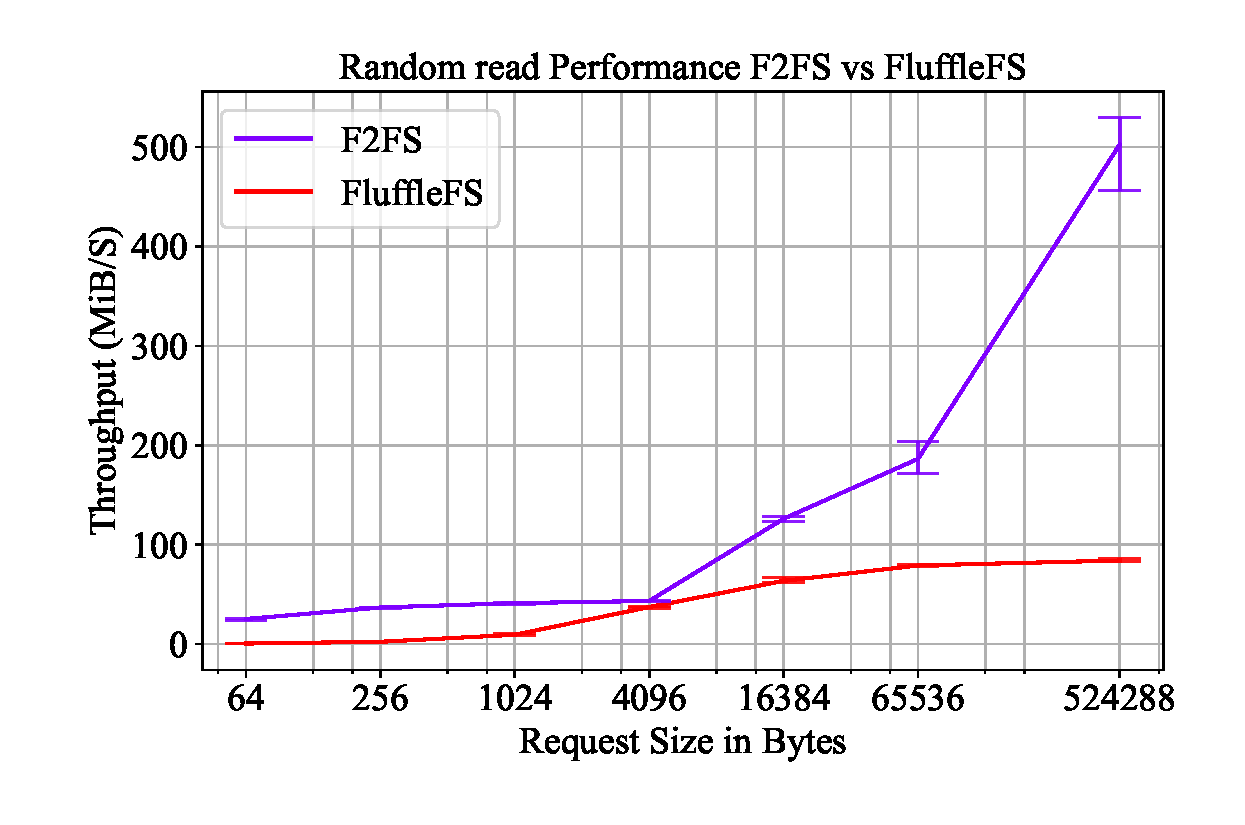
\includegraphics[width=1\textwidth]{resources/images/results-random-read.pdf}
	\caption{Results of random read microbenchmark evaluation using a file size
        of 1GiB}
    % \includesvg[width=0.6\columnwidth]{resources/images/module-dependencies}
    \label{figure:readrandom}
\end{figure}

Regarding random write performance as shown in figure \ref{figure:writerandom}.
Here the performance of FluffleFS is roughly equal to the sequential write
performance. However, F2FS instead has substantially different performance
results. Our first observation is the the random write performance for F2FS is
much higher and more stable with severely smaller difference between the minimum
and maximum. In addition, the mean write performance of F2FS is significantly
higher especially for larger file and request sizes. Most notably is for the
largest results in the sequential and random write benchmarks both file and
request size are identical. Still, the performance difference is substantial and
can only be caused by writing the file sequentially or in random order.

By analysing source code we have determined that F2FS is capable of utilizing
page cache for submitted writes as well as merging incoming I/O requests, writes
and calls to \textit{bio\_put}. Moreover, \textit{bio\_put} is the Linux kernel
block interface and can potentially be used in an asynchronous manner. Given the
large variance observed in write behavior it is likely that write calls complete
before the actual data is flushed to the drive. To investigate how substantially
this write caching influences performance the microbenchmarks can be rerun
using the \textit{O\_DIRECT} and \textit{O\_SYNC} flags upon calling
\textit{open}. Additionally, should the use of these flags proof unsuccessful
the memory contention can be artificially increased by severely limiting the
amount of allocated RAM in virtual machines.

\begin{figure}[h]
    \centering
	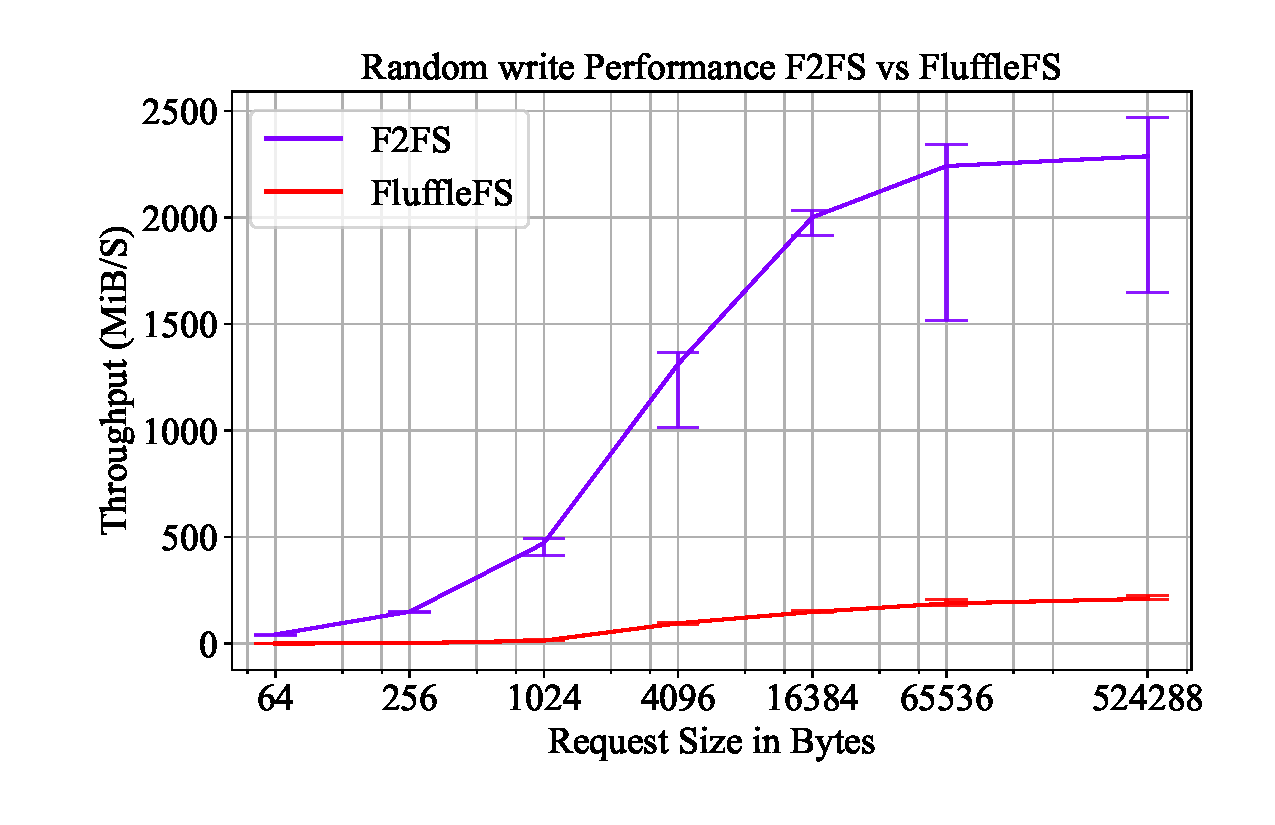
\includegraphics[width=1\textwidth]{resources/images/results-random-write.pdf}
	\caption{Results of random write microbenchmark evaluation using a file size
        of 1GiB}
    % \includesvg[width=0.6\columnwidth]{resources/images/module-dependencies}
    \label{figure:writerandom}
\end{figure}

\subsection{Regular Access Results Discussion}

Similar to sequential reads and writes there is a substantial performance
difference between F2FS and FluffleFS for random reads and writes. Overall the
maximum performance of FluffleFS is considerably low when compared to F2FS. We
have already described three notable differences that might cause such a
performance discrepancy. However, we believe several additional reasons are
further causes of this difference.

Firstly, FUSE based filesystems have to perform additional context switching
between kernel and userspace. A process that has become significantly more
computational intensive due to recently discovered hardware vulnerabilities.
Previous work has shown that between kernel and FUSE based filesystems there can
be a non-negligible performance degradation \cite{Vangoor2017ToFO}. This
degradation was around 83\% in specific workloads with an accompanying increase
in CPU usage of 31\%. However, the minimal performance degradation observed was
just around 5\%.

Secondly, for our specific application the use of inode and data caches as
supported by FUSE had to be explicitly disabled. Otherwise any recent regular
request would influence the return data of an offloaded request if going to the
same region of the same file. It is likely that these inode and data caches are
handled inside the Linux kernel and not by the userspace library of FUSE. 
In the future FluffleFS can likely support inode and data caches by requiring
users to call \textit{open} on offloaded files with the \textit{O\_DIRECT}
flag. However, for our current prototype we have chosen not to investigate this
as this requirement would pose additional barrier to entree.

Third. FluffleFS only submits a single I/O request to the drive moving 4096
bytes per request. This is a very limited method of interacting with the drive
that is likely done substantially differently in F2FS. Not only the performance
differences are evidence that suggests this but explicit management of hot
and cold zones for separate data placement further back this claim.
Additionally, during experimental evaluation the \textit{mq-deadline} I/O
scheduler had to be enabled for the ZNS device to prevent F2FS write errors.
This Linux I/O scheduler serializes outstanding write operations which prevents
the requests inside a ZNS append operation from being reordered. Errors
without the \textit{mq-deadline} scheduler is clear evidence that F2FS submits
multiple I/O requests concurrently.

\subsection{Kernel Passthrough Results}

Our final set of microbenchmarks compare the performance overhead from
offloading to regular access. In addition, we establish the performance impact
on kernels by concurrent regular access. These results are shown in figure
\ref{figure:passthroughresults}. Here we clearly see that the performance
for small file sizes is near identical but starts to diverge more and more
as file size increases. Intuitively we would expect no performance difference
beyond the request size of just 524288 bytes, however, clearly this is not the
case. Most notable is the sudden drop in performance for passthrough beyond
256MiB files. While a similar drop is is observed in the sequential write
performance of F2FS no probable cause is known.

\begin{figure}[h]
    \centering
	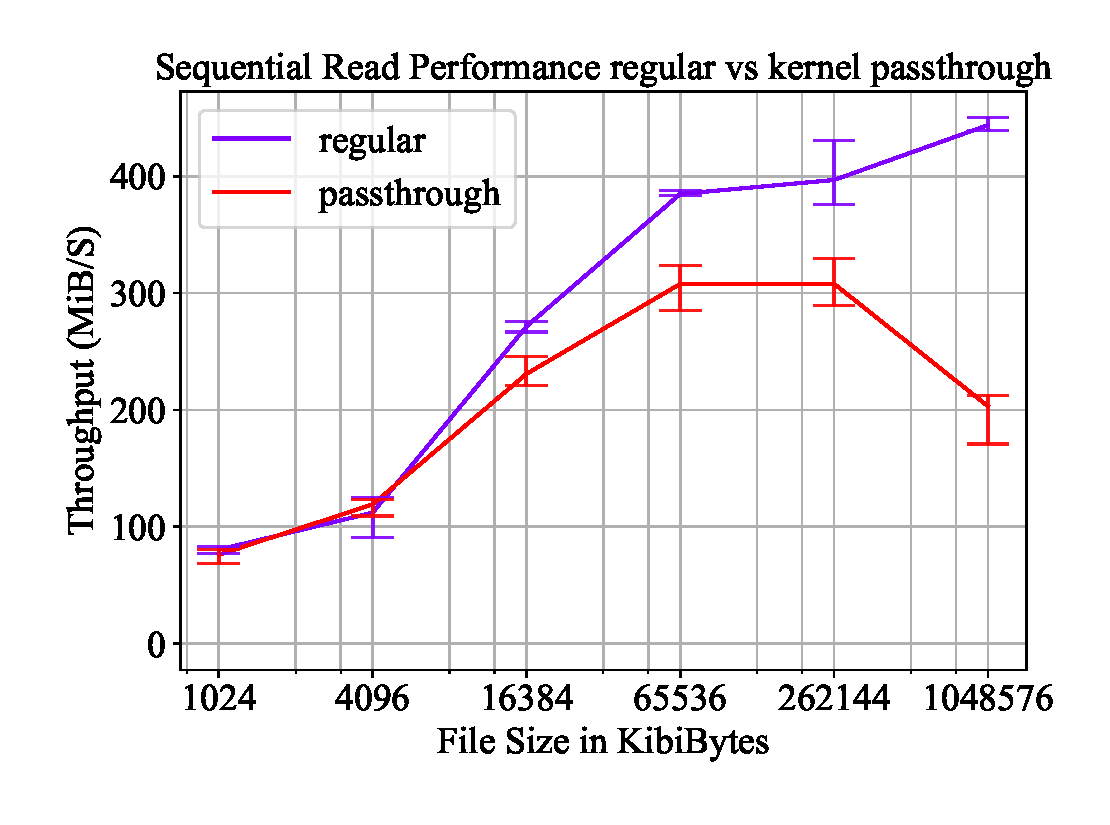
\includegraphics[width=1\textwidth]{resources/images/results-passthrough.pdf}
	\caption{Results Sequential Passthrough}
    % \includesvg[width=0.6\columnwidth]{resources/images/module-dependencies}
    \label{figure:passthroughresults}
\end{figure}

\subsection{Concurrent Access Results}

Our final microbenchmark result is shown in figure
\ref{figure:concurrentpassthrough}. In this figure Dotted lines indicate
baselines from the previous microbenchmark. Furthermore, the red to yellow line
indicates passthrough kernel performance. Contrarily, the blue to cyan line is
used for regular performance. Finally, darker colors represent increasing
numbers of concurrent write jobs scaling from one to four.

From the results shown we can see that both regular and kernel passthrough
performance is still impacted significantly from concurrent write jobs.
However, kernel passthrough has better performance for most file sizes compared
to regular access. These results still show that the concurrent regular and
offloaded access to the same file is able to provide performance benefits.
Unfortunately, we can not conclude that this concurrent performance is entirely
undisturbed. Likely several of the already proposed changes such as submitting
multiple I/O requests concurrently are able to improve concurrent performance
further.

\begin{figure}[h]
    \centering
	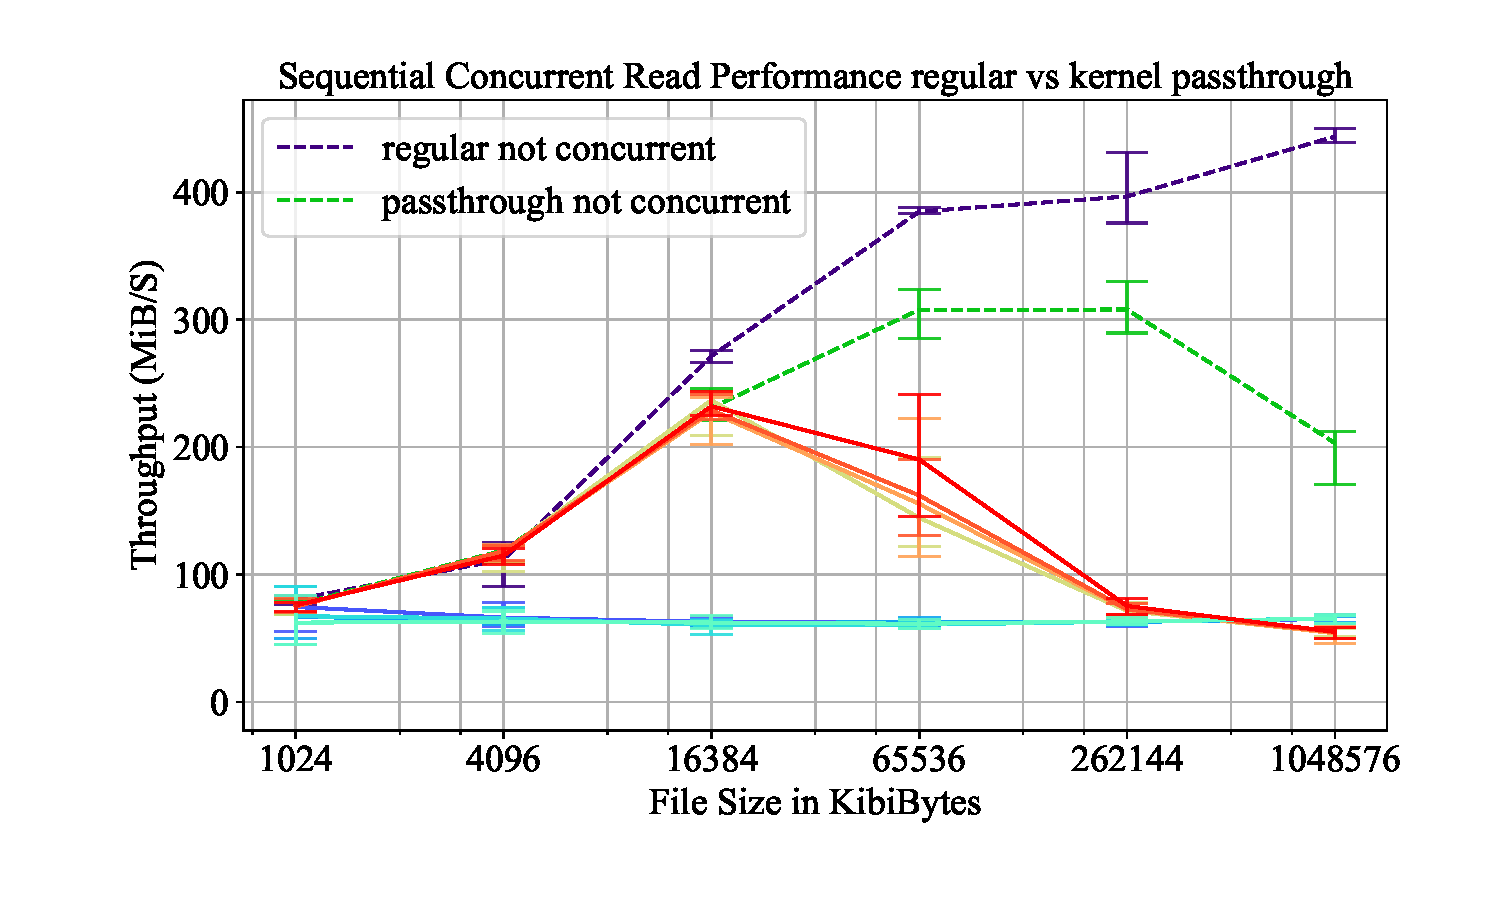
\includegraphics[width=1\textwidth]{resources/images/results-concurrent-read.pdf}
	\caption{Results Concurrent Passthrough.}
    % \includesvg[width=0.6\columnwidth]{resources/images/module-dependencies}
    \label{figure:concurrentpassthrough}
\end{figure}

From these microbenchmarks it is clear that the performance of FluffleFS is
on average significantly lower then top of the line flash optimized filesystem
such as F2FS. However, under a few circumstances both filesystems
performed on par. Given the design requirements and goals of this work this
result is to be expected.

To further improve the performance of this prototype many possible avenues have
been discussed. These are reiterated briefly here. First, I/O requests to
underlying drives  should not be rounded to upper sector size. Second, zero-copy
should be used across interface to reduce data movement. Third, a memory-pool
should be implemented to prevent allocation and de-allocation of memory across
operations. Fourth, inode and data cache functionality should be re-enabled by
requiring the use of the \textit{O\_DIRECT} flag during calls to \textit{open}
when offloading. Fifth, the NVMe backend should be updated to allow multiple
concurrent requests to be submitted to the underlying drive. Finally, the
size of buffers should be increased to allow to move more than 4096 bytes in a
single request.

\section{Shannon Entropy}

In the last results we demonstrate that applications can reduce host CPU load
as well as reduce data movement between the device and host. As discussed the
computation of shannon entropy has been chosen for this.

To evaluate this to implementations to compute shannon entropy are designed.
One written entirely in Python while the other uses Python to combine the
data from individually submitted kernels. Functionality to recombine data from
submitted kernels is necessary as the maximum size of a single I/O request is
524288 bytes (512KiB). For each 512KiB read from the drive only
$256 * 4=1024$ bytes are returned to the host. This constitutes a data reduction
of 1024 times (99.90\%) for this particular application.

In the next two figures the total computation (wall) time of these two
implementations is evaluated using bar graphs. The left hand bar graphs will show
the results for the Python implementation while the right show the offloaded
performance. The total computation time is divided into three categories being
time spent in userspace (user), time spent in kernelspace (sys) and time spent
waiting (wait). Notably, during the time spent in wait the kernel can assign
other processes to run instead reducing CPU host load. Finally, as before the
error bars indicate the minimum and maximum observed difference across all 30
measurements. The results are shown in figures \ref{figure:shannonlow} and
\ref{figure:shannonhigh} for smaller and larger file sizes respectively. Please
Note that the vertical axis between both figures have substantially different
scales.

\begin{figure}[h]
    \centering
	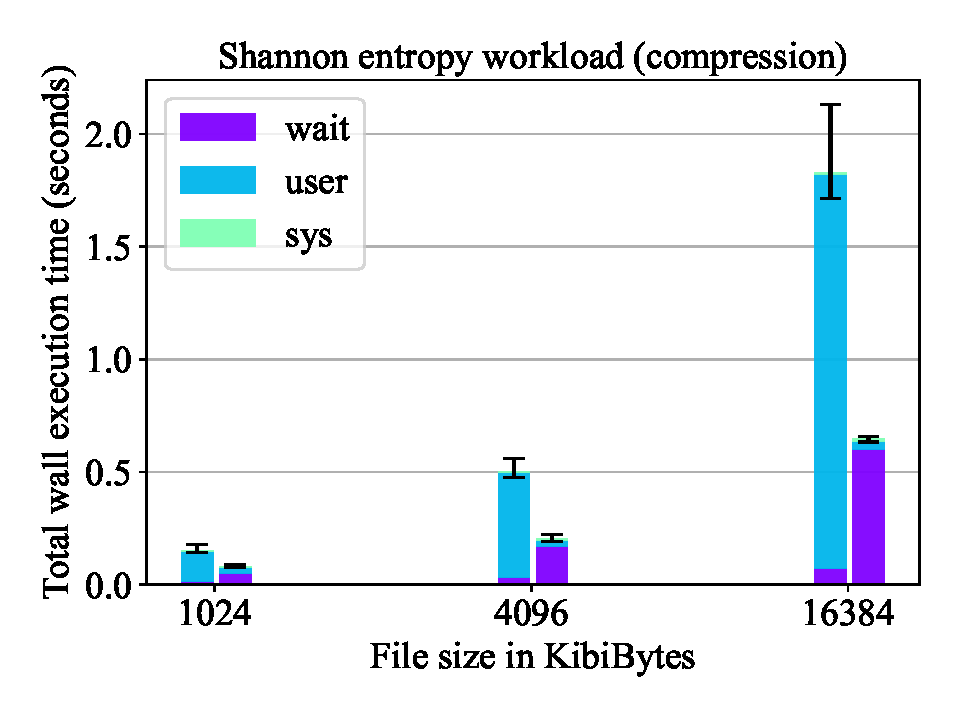
\includegraphics[width=1\textwidth]{resources/images/results-shannon-lower.pdf}
	\caption{Wall time across different contexts for larger file sizes}
    % \includesvg[width=0.6\columnwidth]{resources/images/module-dependencies}
    \label{figure:shannonlow}
\end{figure}

\begin{figure}[h]
    \centering
	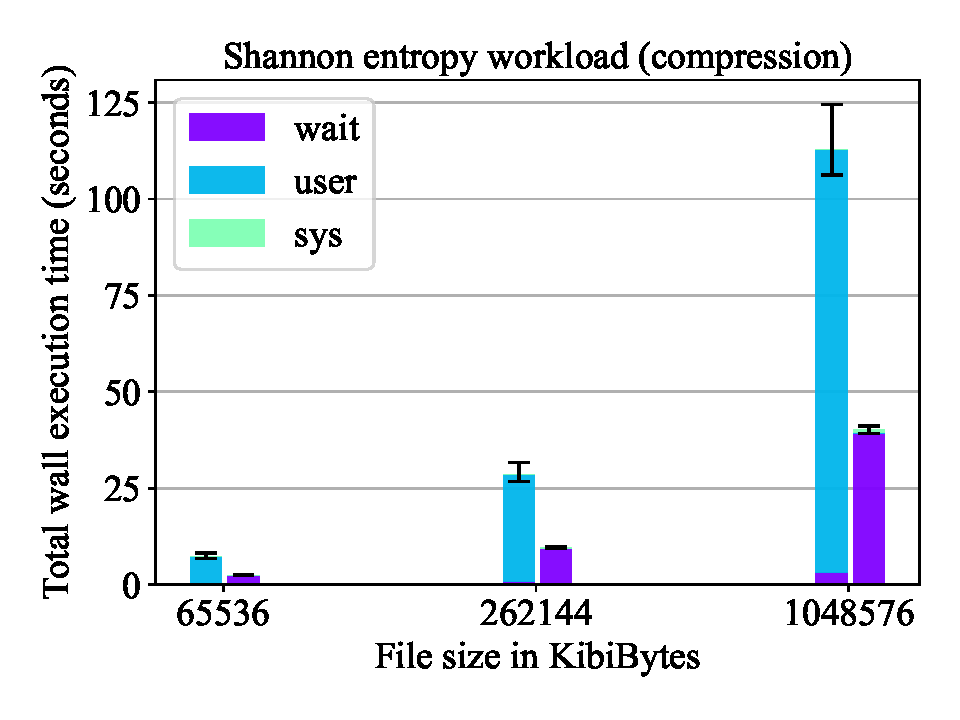
\includegraphics[width=1\textwidth]{resources/images/results-shannon-upper.pdf}
	\caption{Results Sequential Passthrough}
    % \includesvg[width=0.6\columnwidth]{resources/images/module-dependencies}
    \label{figure:shannonhigh}
\end{figure}

Across all these results unanimously our kernel offloaded implementation
is faster compared to our Python implementation. While this not the main goal of
this experiment it is good to see that eBPF \& uBPF can achieve good
performance when using JiT compilation. However, it should be noted that
a fairer comparison would have evaluated a C or C++ implementation against our
offloaded kernel.

Lower execution time inherently reduces the host CPU load. However, this is not
the main observation from these results. Far more important is how almost the
entire execution time of the offloaded application is spent in wait state.
Meaning, that the host CPU is free to perform other tasks while waiting from the
results of the CSx.

Together these results demonstrate that a hybrid filesystem supporting
concurrent regular and offloaded access is able to reduce data movement between
host and device as well as reduce host CPU load in asynchronous applications.

% \subsection{Normalization}

% The compute capabilities of embedded devices such as those that will
% be found on NVMe SSDs and future CSxs is significantly lower compared to the
% host CPU. Will this might change in the future we would have liked to normalize
% our results by differentiating the compute capabilities between the host and
% a commonly found embedded device. Unfortanetely, no vendor releases information
% about the compute capabilities of their NVMe controllers, at least without a
% \textit{Non-Disclosure Argeement} (NDA). Instead we turn to commercially
% available CSxs such as the NGD newport utlizing available literature
% \cite{10.1145/3415580} to estimate the performance of compute cores.

% From this work it can be shown that a NGD newport device contains four ARM A53
% cores that achieve 2.3 DMIPS/MHz. The operating frequency of these cores must be
% between 0.957 and 2.65 GHz. The Dmips performance indication is evaluated using
% a dhrystone benchmark that does not use floating point arithmatic. This is the
% most relavent performance metric available as the computation of shannon entropy
% does not use floating point arithmatic either. Furthermore, the floating point
% capabilities of eBPF are very limited requiring the manual implementation of
% fixed point arithmatic to be performed at all. However, the use of MIPS as 
% performance metric is highly debated as it often is a poor indicator.
% Altneratively, llvm-mca \cite{llvm-mca} can be used to more accurately model the
% number of CPU cycles the kernel would take on each architure. Unfortunately,
% this could not be performed for this normalization due to time constraints.

% Dhrystone 2 using register variables       42381094.2 lps   (10.0 s, 7 samples)

% ---------------------------------------------------------------------------
% ----------------------- end of thesis sub-document ------------------------
% ---------------------------------------------------------------------------

% this file is called up by thesis.tex
% content in this file will be fed into the main document

\chapter{Discussion} % top level followed by section, subsection


% ----------------------- paths to graphics ------------------------

% change according to folder and file names
\ifpdf
    \graphicspath{{7/figures/PNG/}{7/figures/PDF/}{7/figures/}}
\else
    \graphicspath{{7/figures/EPS/}{7/figures/}}
\fi


% ----------------------- contents from here ------------------------
% 

\dots



% ---------------------------------------------------------------------------
% ----------------------- end of thesis sub-document ------------------------
% ---------------------------------------------------------------------------

\chapter{Conclusion}

To conclude, we have demonstrated that many previous prototype for flash based
CSxs exist and have been developed in the past decade. Until now, none of
these prototype where able to provide concurrent regular and offloaded
filesystem access, aptly named \textit{hybrid filesystems}. Our simulation
framework \textit{OpenCSD} and filesystem \textit{FluffleFS} are able to perform
offloading entirely using existing APIs, no shared libraries or network
communication is necessary. In addition, our kernels are vendor agnostic and
filesystem aware. Finally, our prototype runs entirely in userspace requiring no
understanding of the Linux kernel or modifications.

To do this our offloading is triggered through filesystem extended attributes
resulting in complete isolation from regular operating system behavior. These
filesystem extended attributes are present in all modern operating systems
including Windows, MacOs, FreeBSD and Linux. Across all previous CSx works only
a single other work managed to use existing APIs and in doing so they changed
UNIX pipe behavior \cite{10.1145/3342195.3387557}.

Concurrent regular and offloaded access is achieved by utilizing snapshot
consistency with LFS and ZNS technologies. Furthermore,
by utilizing eBPF and uBPF these kernels written for offloading can be made
vendor and filesystem agnostic. While the API for kernel filesystem support
still needs to be formalized and the proposed CSx runtime is still absent in our
prototype, the possibility of filesystem awareness in a concurrent regular and
offloaded setting has been proven. Furthermore we have proven that regular and
offloaded accesses can be easily differentiated utilized PID inode pairs.

Throughout this work we have argued why LFS, ZNS, eBPF and extended attributes
are the current best suited technologies to implement a hybrid filesystem.

We believe that many CSx prototype suffer from a high barrier to entree due to
complicated setup and technologies. Therefor, our design focussed heavily on
being easy to use to reduce barrier to entree. Our design has achieved this by
only utilizing userspace technologies, requiring no knowledge of kernel
development or any kernel modifications. In addition, our framework
\textit{OpenCSD} utilizes a component architecture that easily allows for
replacement of used technologies.

During the evaluation we showed that offloaded applications can reduce
data movement between the device and host by 99.9\% as well as drastically
reduce the host CPU load. However, the overall performance of FluffleFS still
needs to be improved significantly, only able to perform on par with flash
optimized filesystems under very select circumstances. Furthermore, our
limited performance optimizations made us unable to proof that concurrent
offloaded and regular file access can achieve unstagnated performance.

We encourage everyone to try our prototype today which is readily available
and open-source published under a permissive license \cite{qemu-csd}. Along our
source code are datasets of our measurements as well as the scripts to perform
these measurements and generate accompanying graphs. Even the source files for
this very thesis are included. We hope this openness inspires others to do the
same.

% ---------------------------------------------------------------------------
% ----------------------- end of thesis sub-document ------------------------
% ---------------------------------------------------------------------------
          
% this file is called up by thesis.tex
% content in this file will be fed into the main document

%: ----------------------- name of chapter  -------------------------
% \chapter*{Appendix} % top level followed by section, subsection


% %: ----------------------- paths to graphics ------------------------

% % change according to folder and file names
% \ifpdf
%     \graphicspath{{X/figures/PNG/}{X/figures/PDF/}{X/figures/}}
% \else
%     \graphicspath{{X/figures/EPS/}{X/figures/}}
% \fi

%: ----------------------- contents from here ------------------------
% \includepdf[pages=1-5]{CodesTable}
% \includepdf[pages=1-4]{InterviewQuestions}

% ---------------------------------------------------------------------------
%: ----------------------- end of thesis sub-document ------------------------
% ---------------------------------------------------------------------------


      
            
% --------------------------------------------------------------
%:                  BACK MATTER: appendices, refs,..
% --------------------------------------------------------------

% the back matter: appendix and references close the thesis


%: ----------------------- bibliography ------------------------

% The section below defines how references are listed and formatted
% The default below is 2 columns, small font, complete author names.
% Entries are also linked back to the page number in the text and to external URL if provided in the BibTex file.

% PhDbiblio-url2 = names small caps, title bold & hyperlinked, link to page 
%\begin{multicols}{2} % \begin{multicols}{ # columns}[ header text][ space]
%\begin{tiny} % tiny(5) < scriptsize(7) < footnotesize(8) < small (9)

\bibliographystyle{Latex/Classes/PhDbiblio-url2} % Title is link if provided
\renewcommand{\bibname}{References} % changes the header; default: Bibliography

\bibliography{11_references/references.bib} % adjust this to fit your BibTex file

%\end{tiny}
%\end{multicols}



% --------------------------------------------------------------
% Various bibliography styles exit. Replace above style as desired.

% in-text refs: (1) (1; 2)
% ref list: alphabetical; author(s) in small caps; initials last name; page(s)
%\bibliographystyle{Latex/Classes/PhDbiblio-case} % title forced lower case
%\bibliographystyle{Latex/Classes/PhDbiblio-bold} % title as in bibtex but bold
%\bibliographystyle{Latex/Classes/PhDbiblio-url} % bold + www link if provided

%\bibliographystyle{Latex/Classes/jmb} % calls style file jmb.bst
% in-text refs: author (year) without brackets
% ref list: alphabetical; author(s) in normal font; last name, initials; page(s)

%\bibliographystyle{plainnat} % calls style file plainnat.bst
% in-text refs: author (year) without brackets
% (this works with package natbib)


% --------------------------------------------------------------

% according to Dresden med fac summary has to be at the end
%
% Thesis Abstract -----------------------------------------------------


%\begin{abstractslong}    %uncommenting this line, gives a different abstract heading
\begin{abstracts}        %this creates the heading for the abstract page

Here goes the abstract of this thesis.
\end{abstracts}
%\end{abstractlongs}


% ---------------------------------------------------------------------- 


%: Declaration of originality
%\include{8_backmatter/declaration}



\end{document}
